On June 30th, 2018, a false fire alarm at Point 5 on the LHC triggered temporary power disruptions to CMS, resulting in two dead HCAL wedges in the minus endcap for the duration of 2018. The failed wedges, HEM 15 and 16, occupy a \SI{40}{\degree} region in the detector, specifically $-3.0 < \pseudorap < -1.3$ and $-1.57 < \phi < -0.87$. The affected runs begin with run 319077 until the end of 2018. A study is performed to ensure the HEM 15/16 failure does not impact any kinematic distributions used in this analysis. 2018 data are divided into two periods: A and B, corresponding to all runs before run 319077 and all runs after and including run 319077, respectively. After preselection is applied, kinematic distibutions for each data period are normalized to unity so a shape comparison can be performed. No significant difference in shape is observed in any disributions in periods A and B.

\begin{figure}[H]
    \centering
    {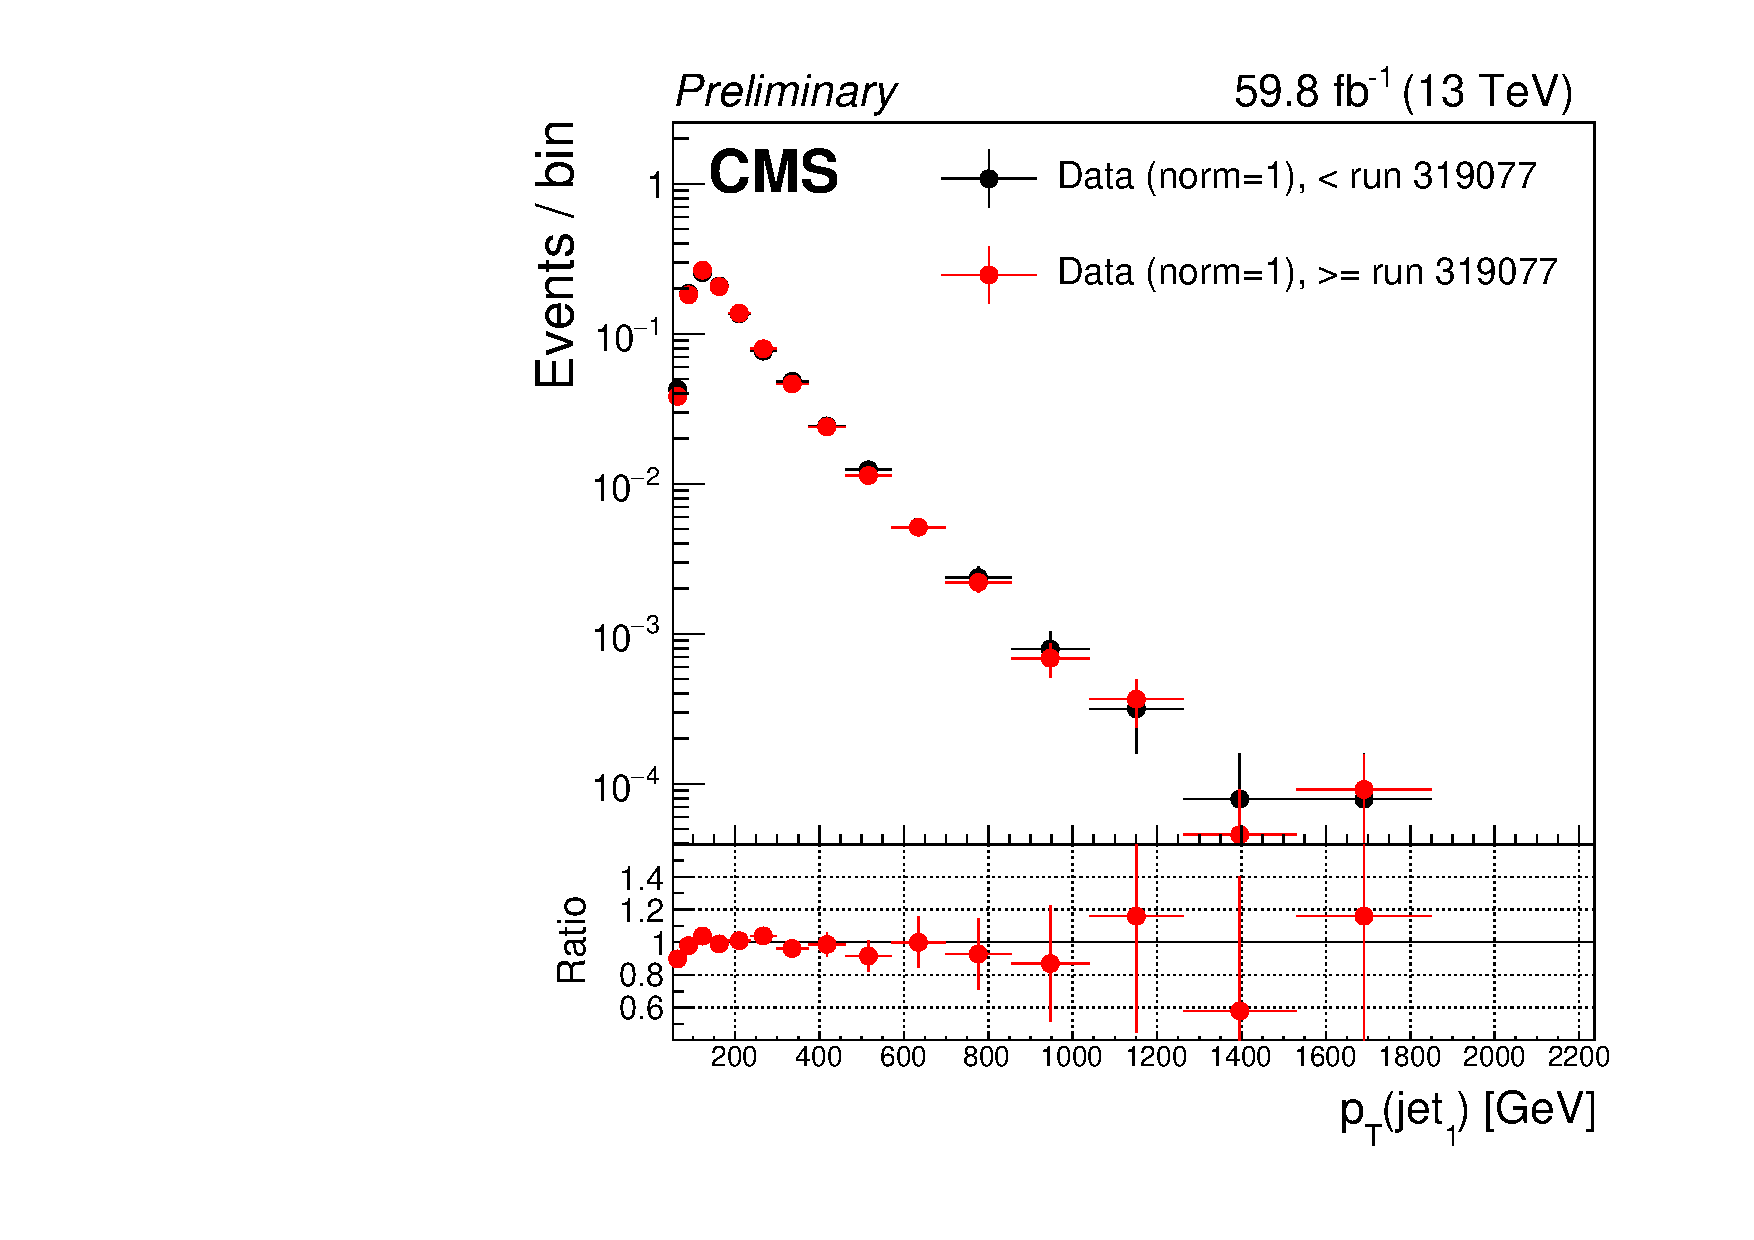
\includegraphics[width=.49\textwidth]{Images/Analysis/Results_HEMFailureStudyPlots_Data_BeforeAfterRun319077/BasicLQ_uujj_Pt_jet1_standard.pdf}}
    {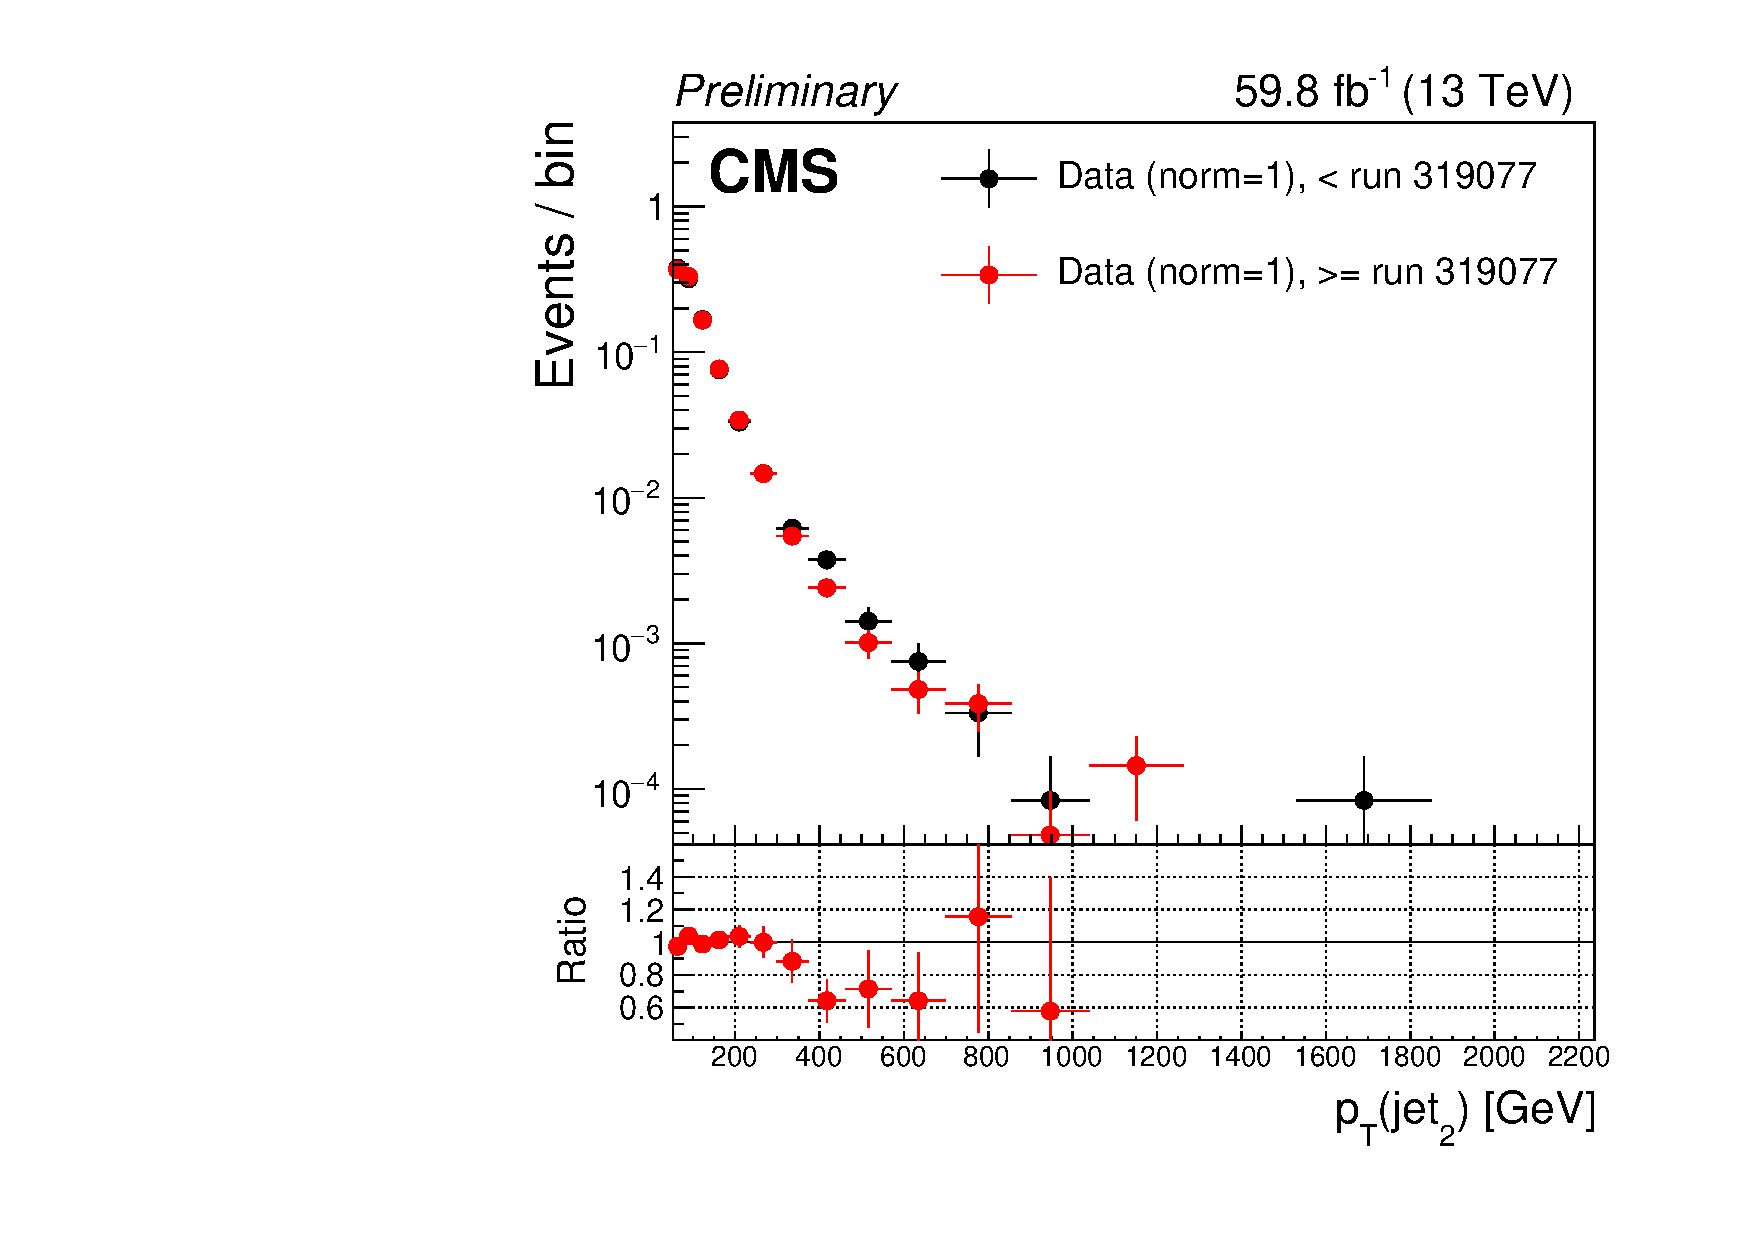
\includegraphics[width=.49\textwidth]{Images/Analysis/Results_HEMFailureStudyPlots_Data_BeforeAfterRun319077/BasicLQ_uujj_Pt_jet2_standard.pdf}}
    {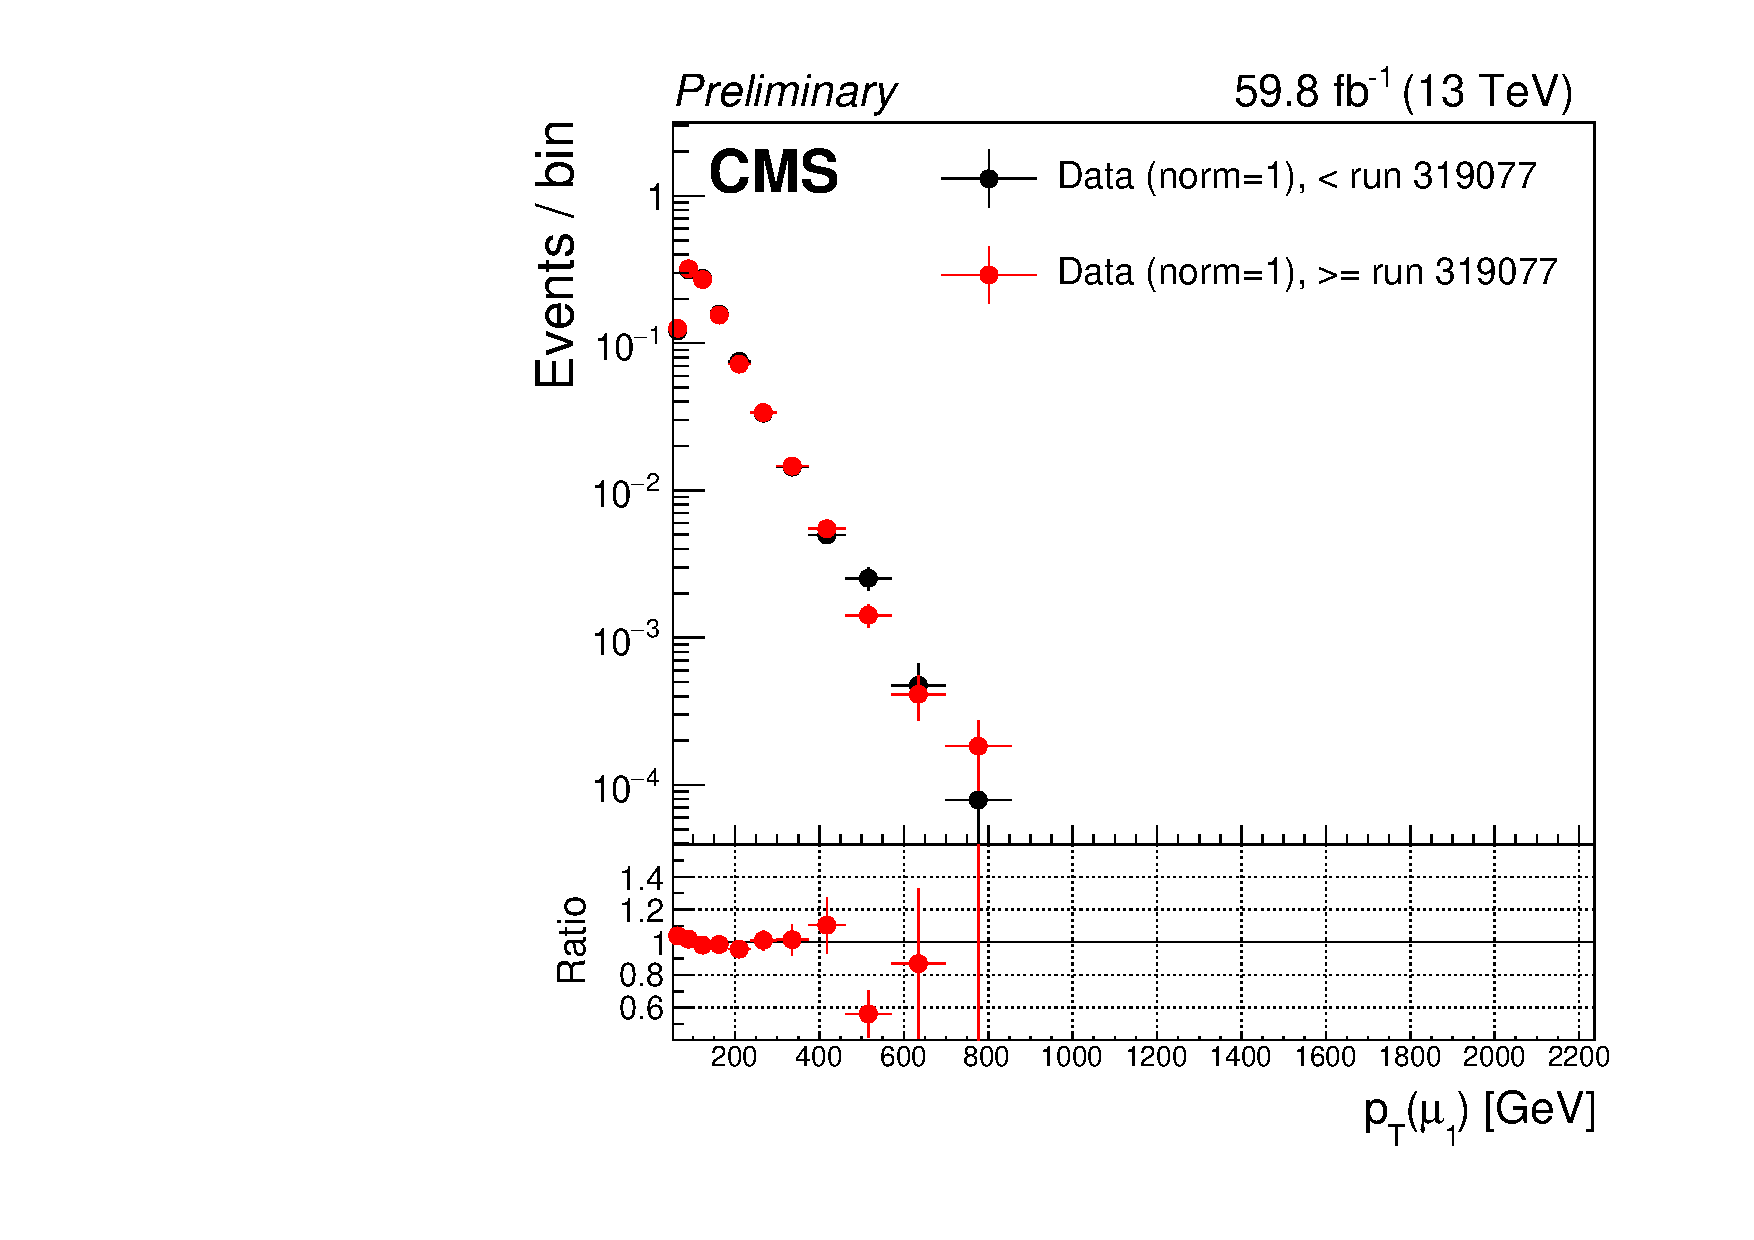
\includegraphics[width=.49\textwidth]{Images/Analysis/Results_HEMFailureStudyPlots_Data_BeforeAfterRun319077/BasicLQ_uujj_Pt_muon1_standard.pdf}}
    {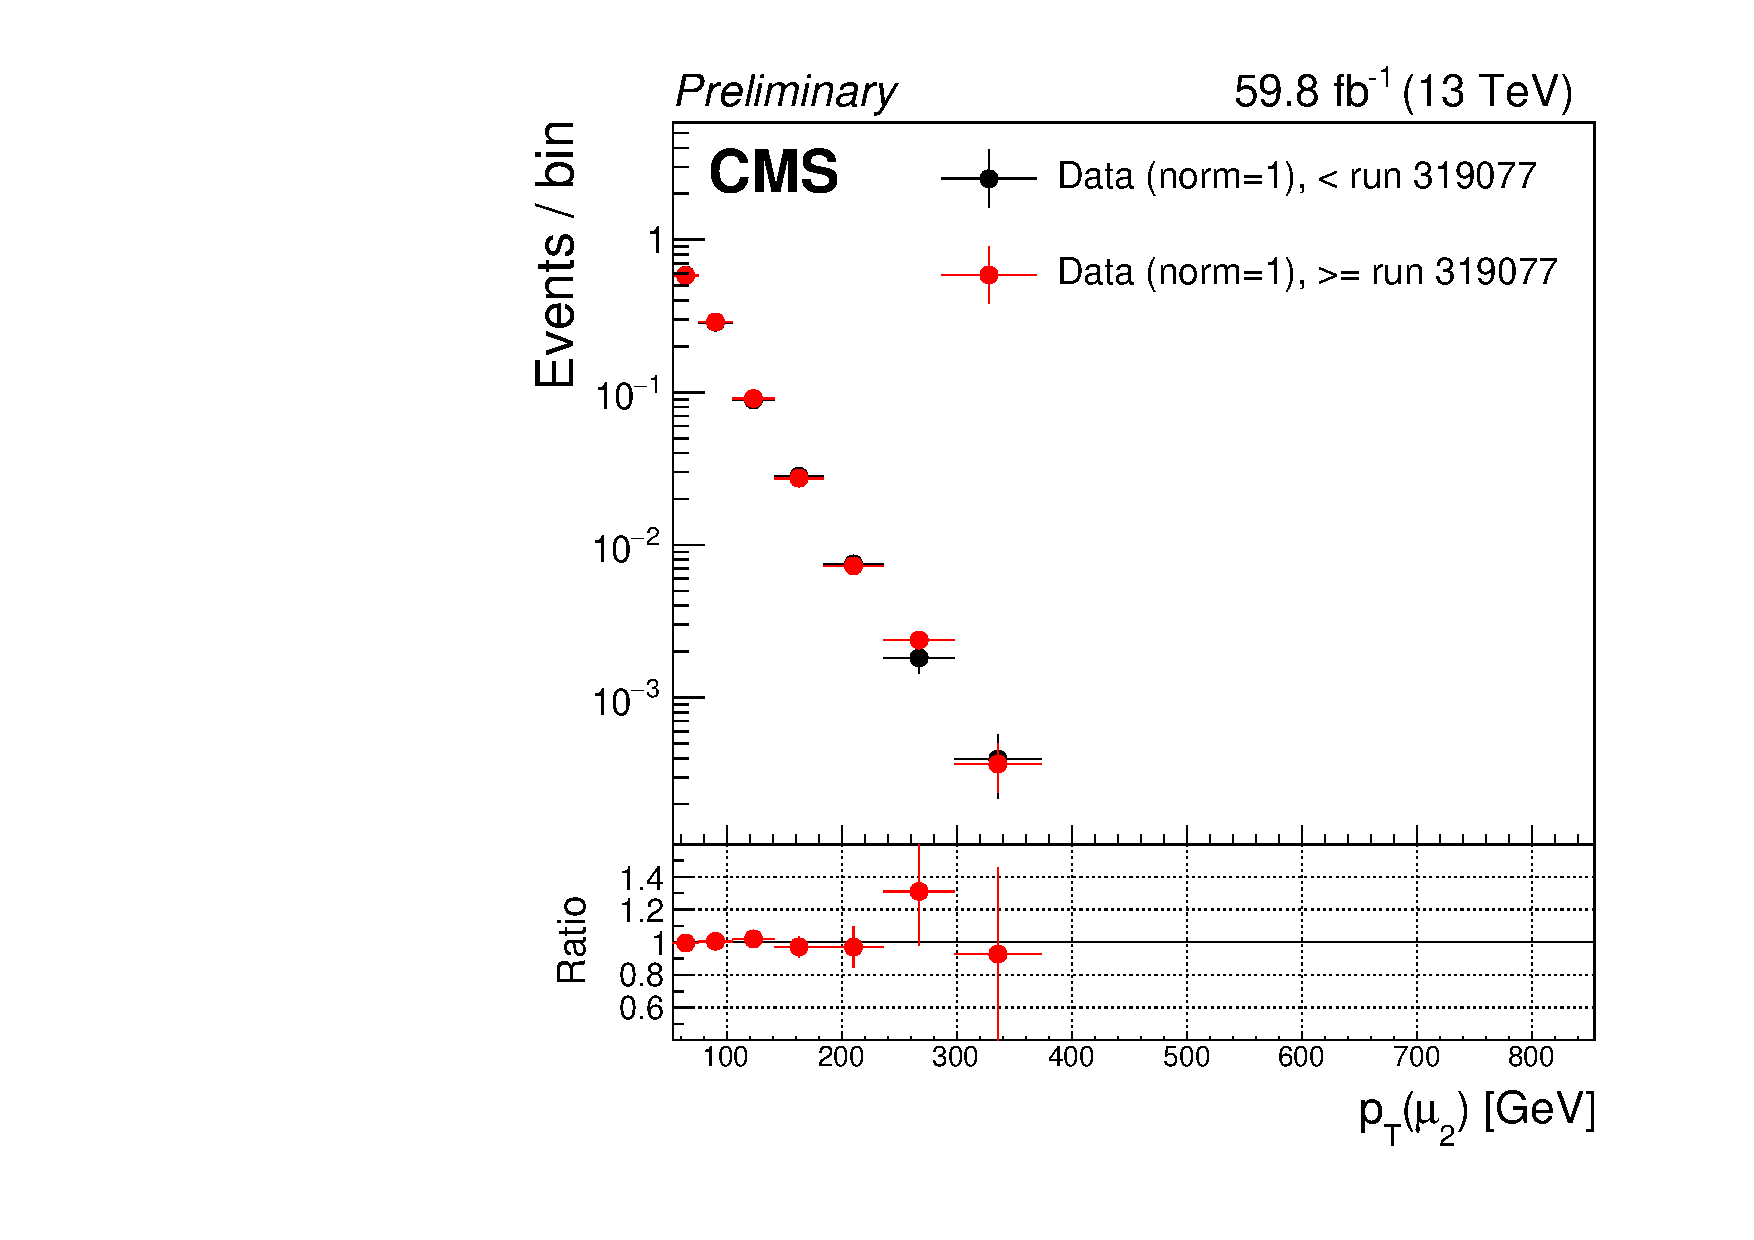
\includegraphics[width=.49\textwidth]{Images/Analysis/Results_HEMFailureStudyPlots_Data_BeforeAfterRun319077/BasicLQ_uujj_Pt_muon2_standard.pdf}}
    \caption{A shape comparison of 2018 data in periods A (black) and B (red). Data in each period have been normalized to unity and have preselection applied. The ratio \RatioDataAB is shown in the subplot. Vertical error bars represent the statistical uncertainty in each bin.}
    \label{figapp:hemjetmuonpt}
\end{figure}

\begin{figure}[H]
    \centering
    {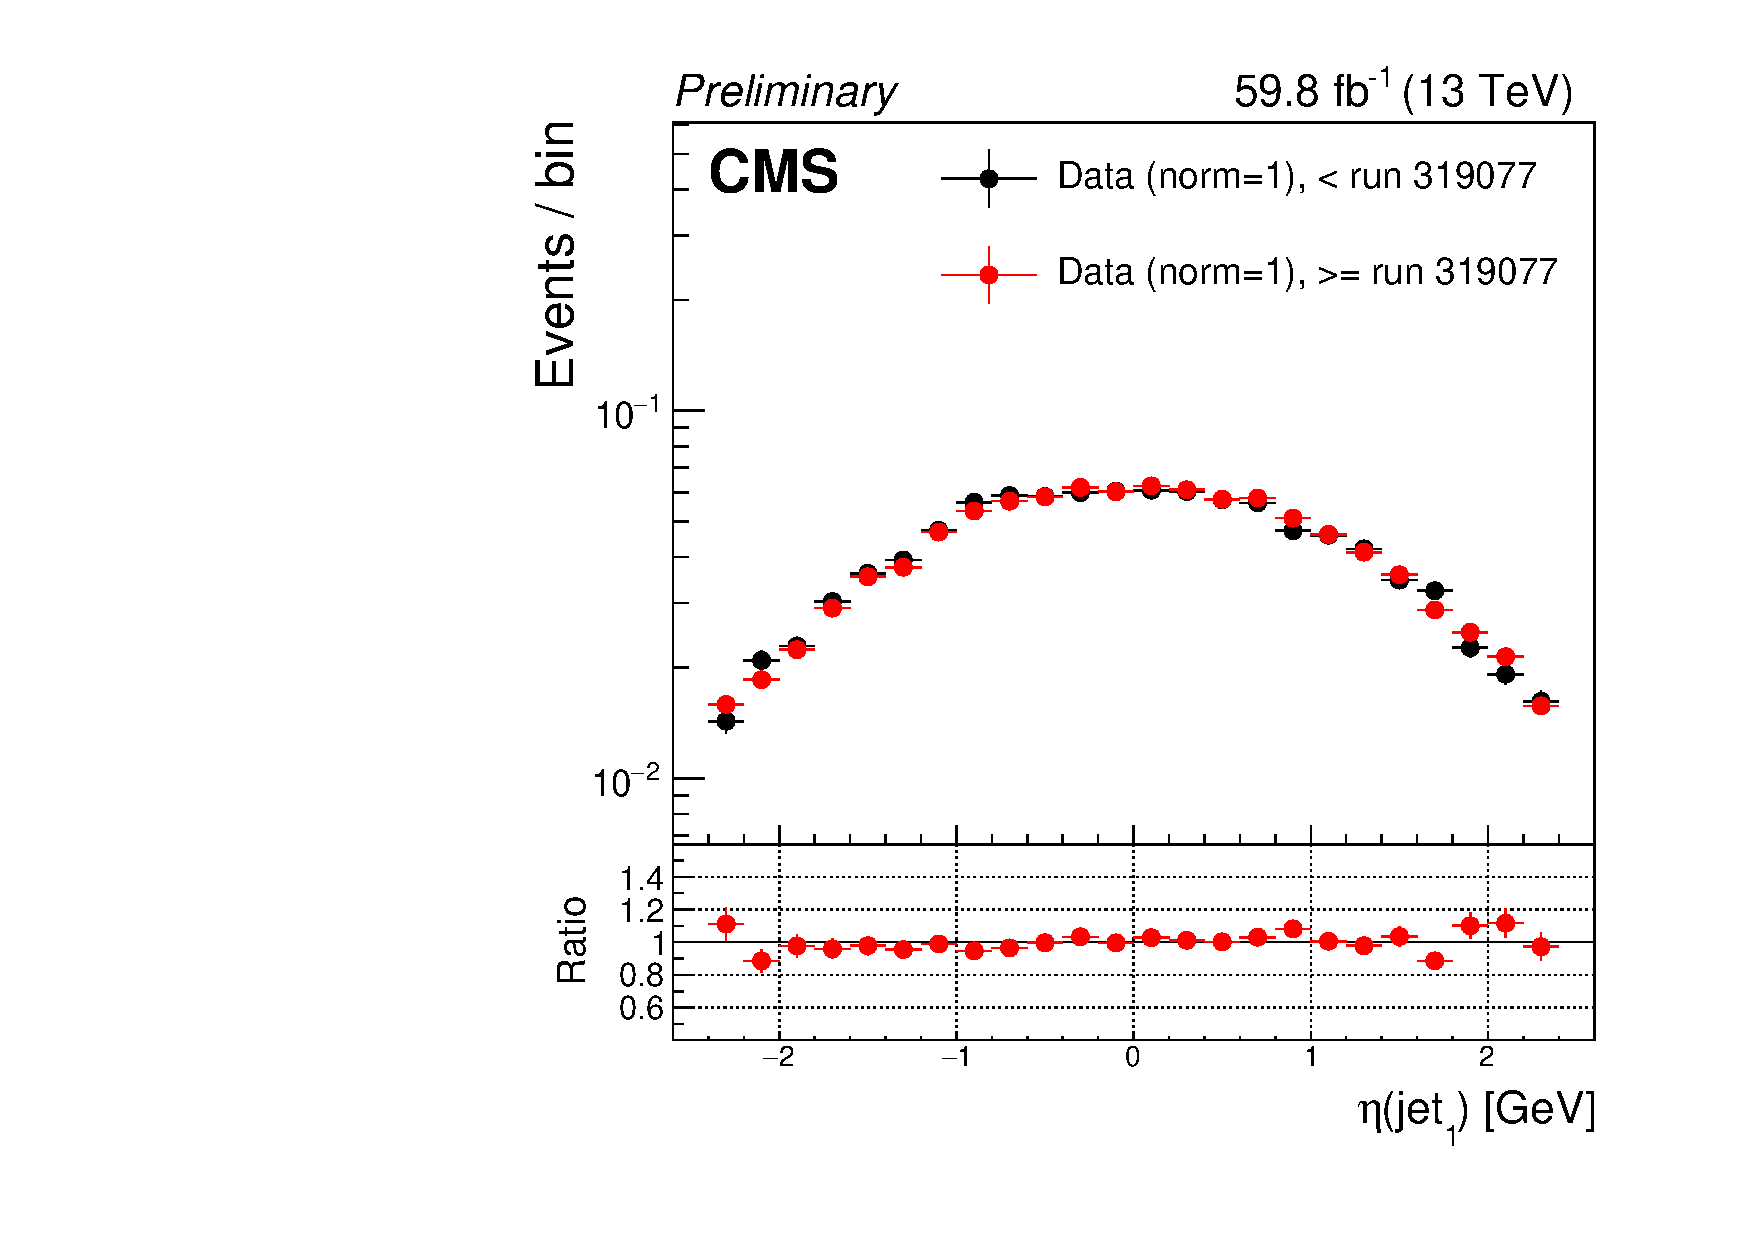
\includegraphics[width=.49\textwidth]{Images/Analysis/Results_HEMFailureStudyPlots_Data_BeforeAfterRun319077/BasicLQ_uujj_Eta_jet1_standard.pdf}}
    {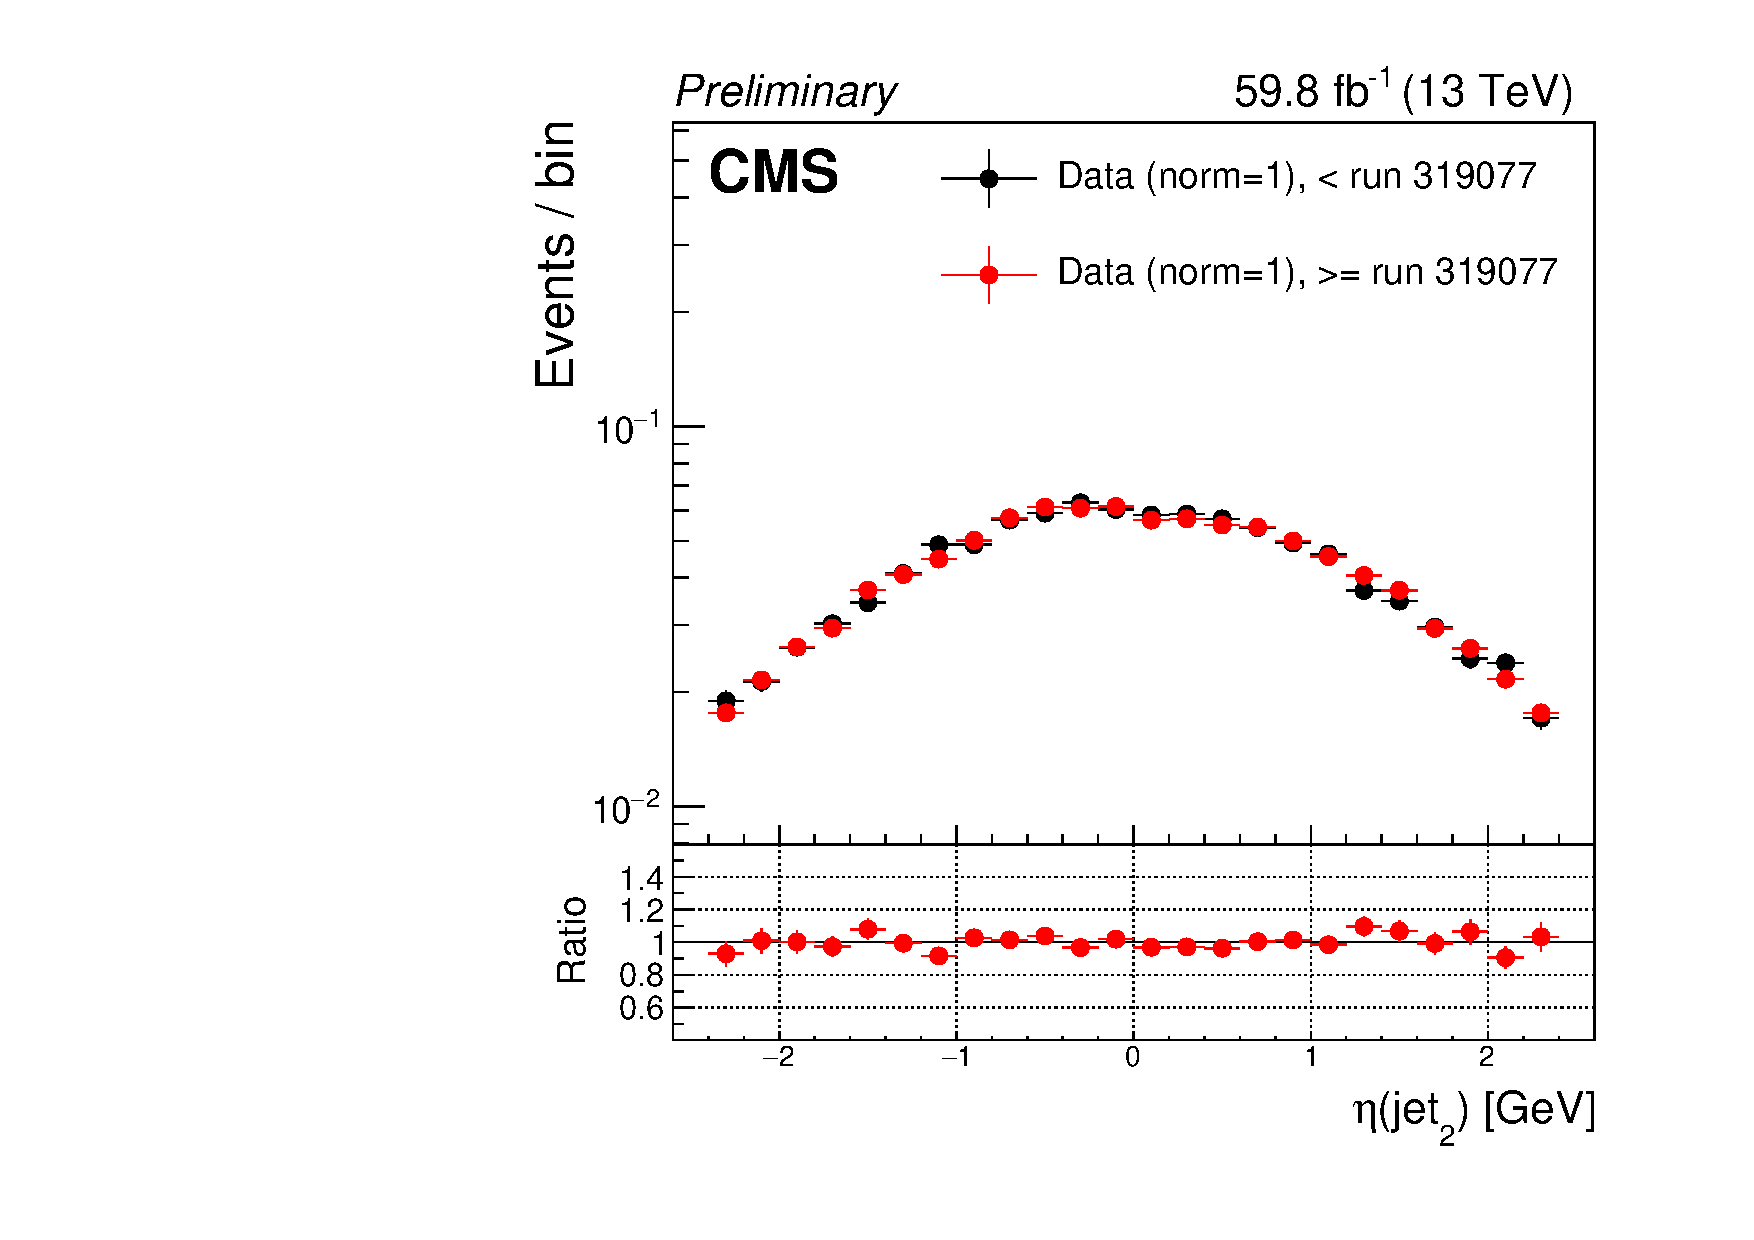
\includegraphics[width=.49\textwidth]{Images/Analysis/Results_HEMFailureStudyPlots_Data_BeforeAfterRun319077/BasicLQ_uujj_Eta_jet2_standard.pdf}}
    {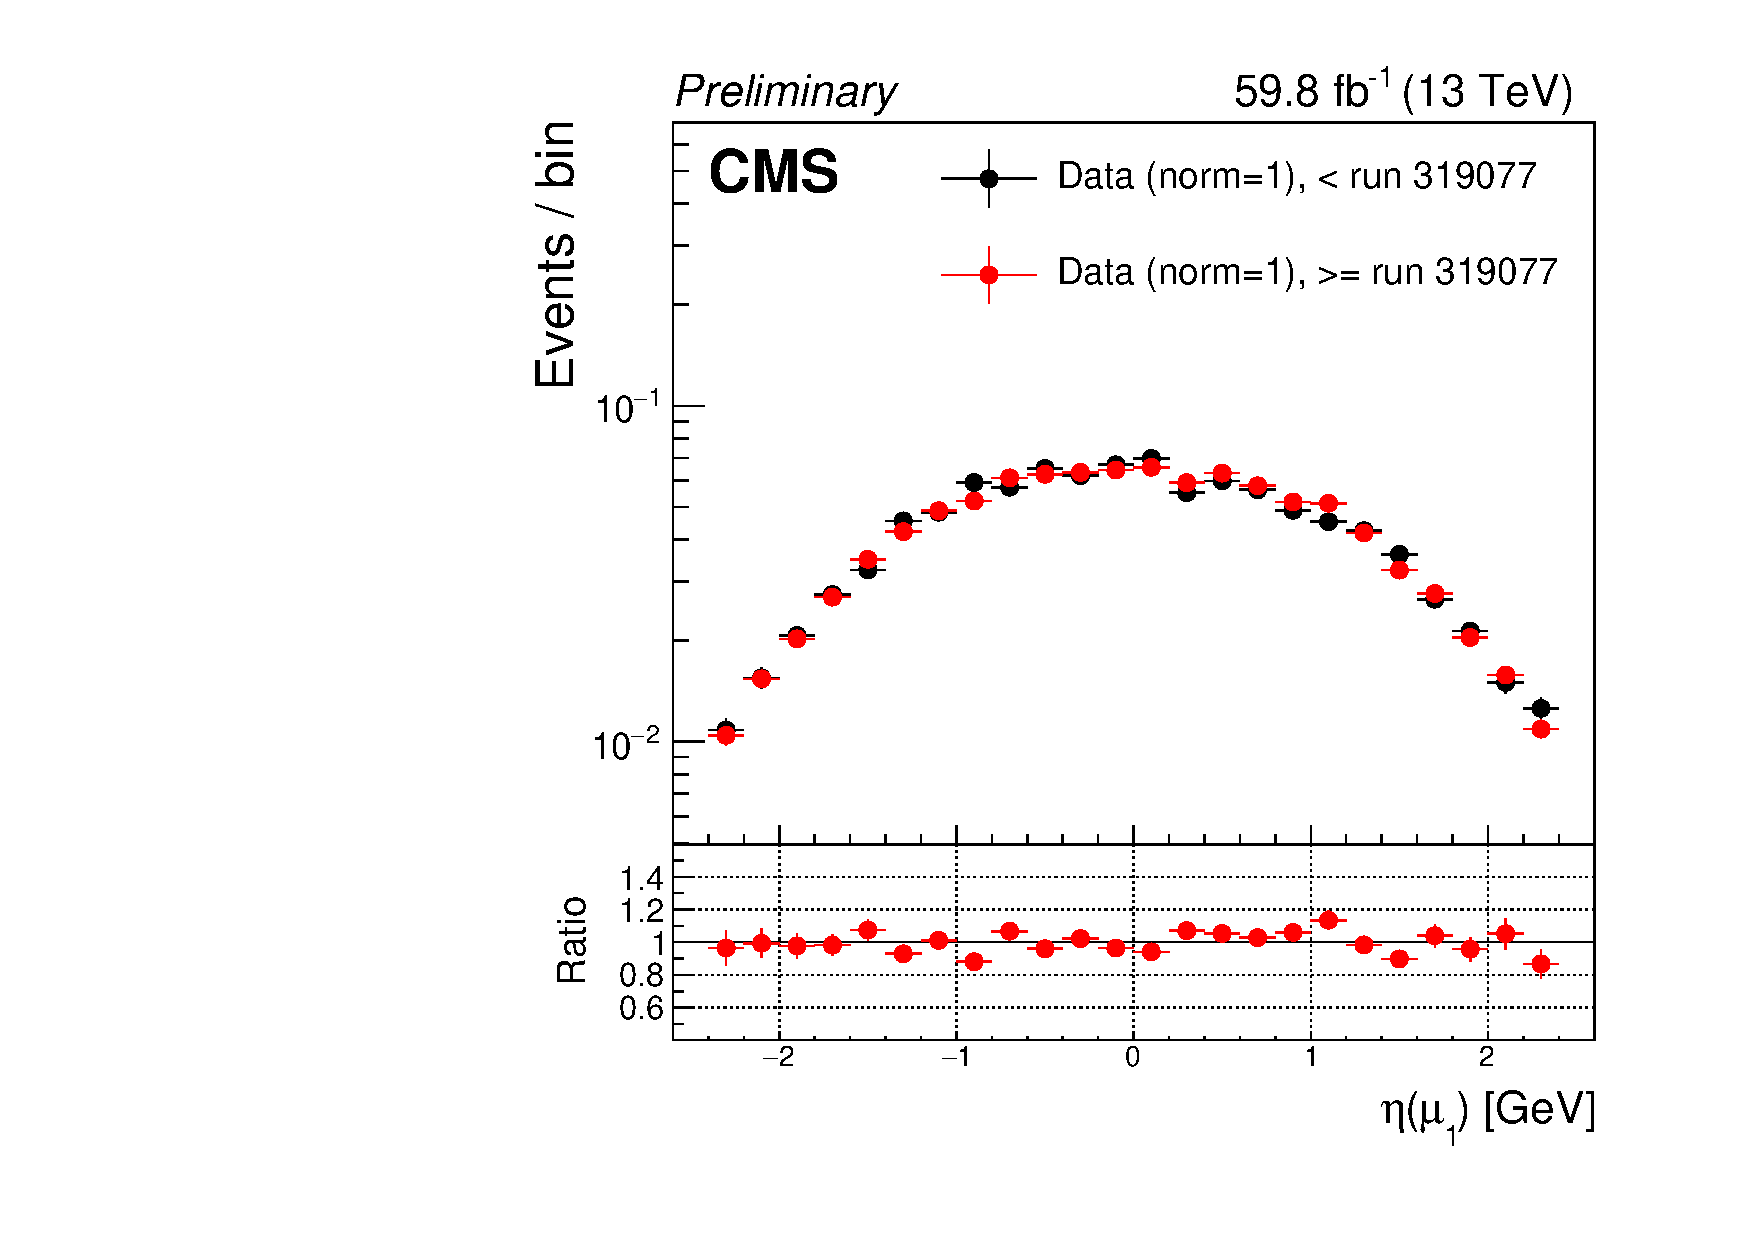
\includegraphics[width=.49\textwidth]{Images/Analysis/Results_HEMFailureStudyPlots_Data_BeforeAfterRun319077/BasicLQ_uujj_Eta_muon1_standard.pdf}}
    {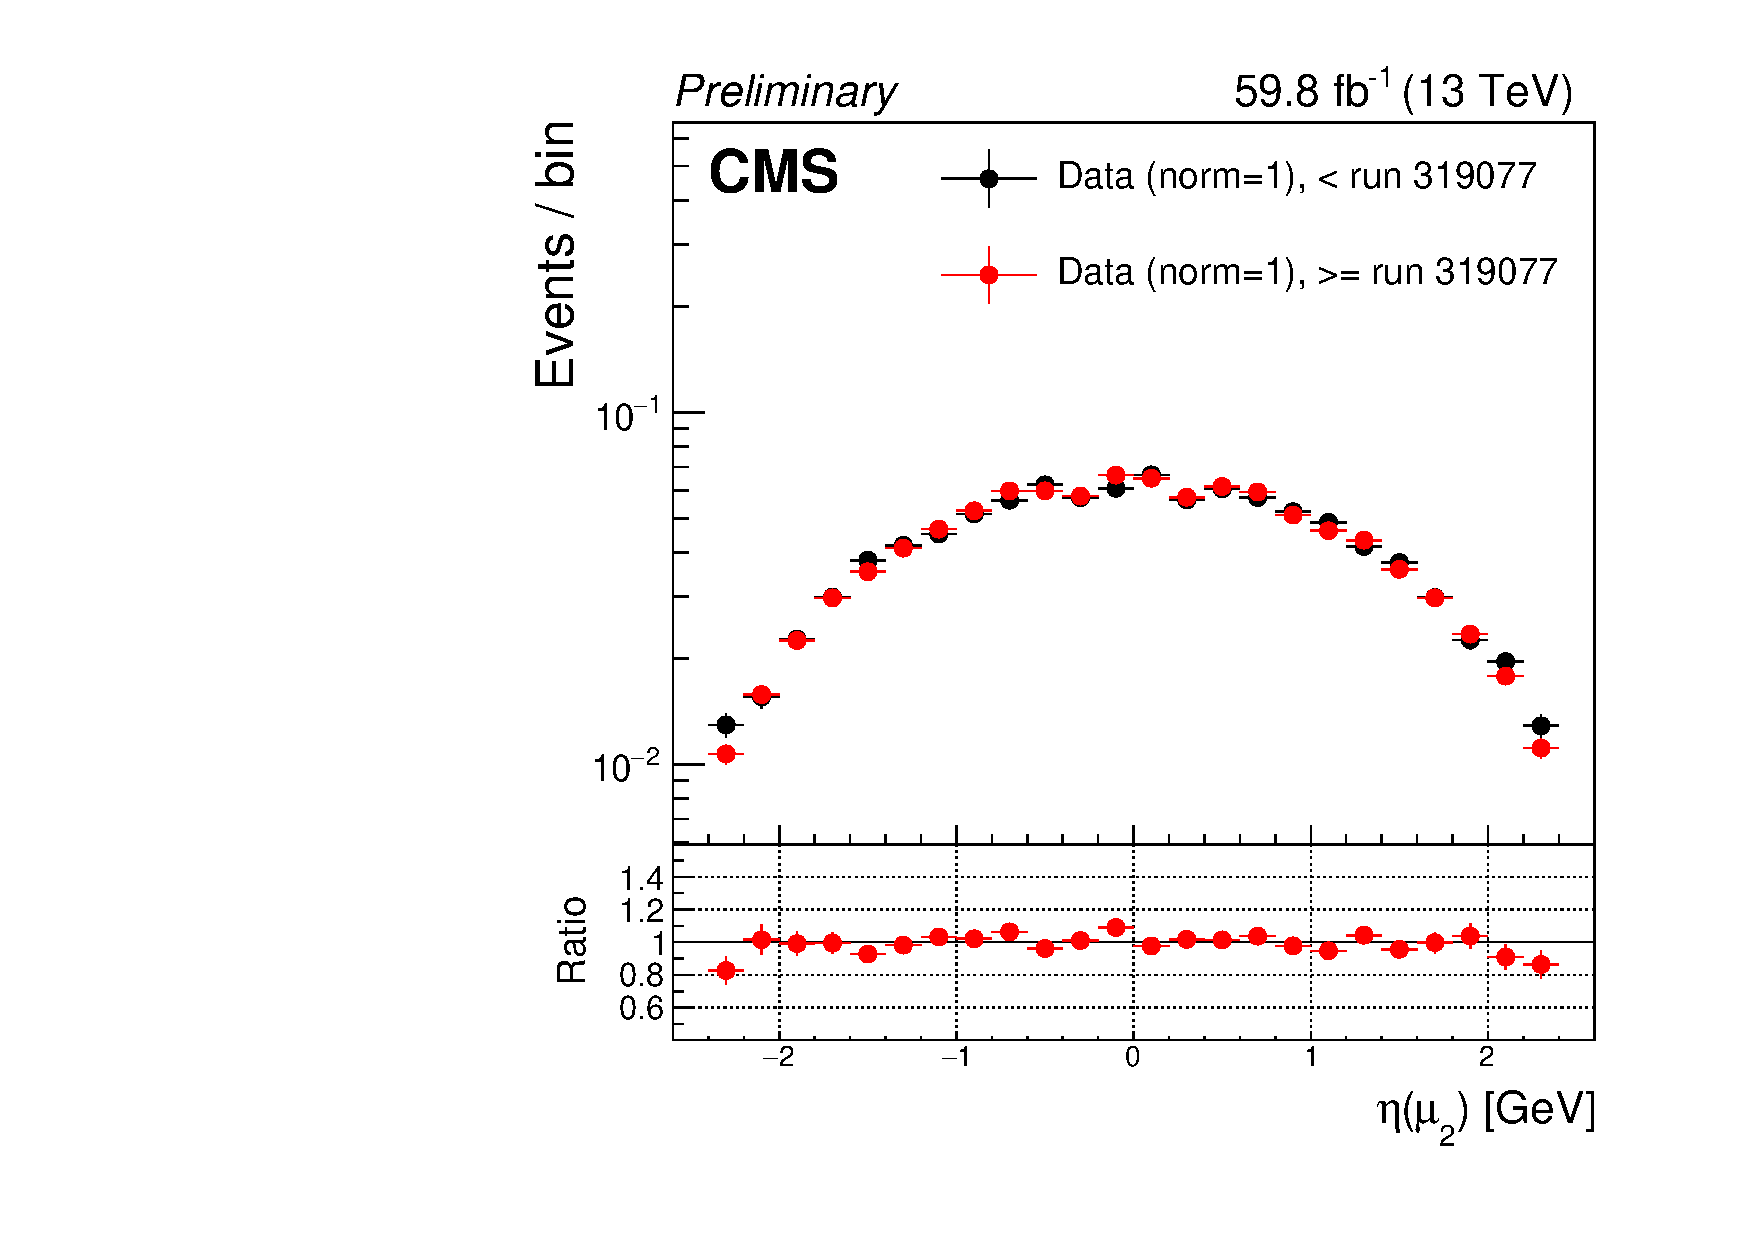
\includegraphics[width=.49\textwidth]{Images/Analysis/Results_HEMFailureStudyPlots_Data_BeforeAfterRun319077/BasicLQ_uujj_Eta_muon2_standard.pdf}}
    \caption{A shape comparison of 2018 data in periods A (black) and B (red). Data in each period have been normalized to unity and have preselection applied. The ratio \RatioDataAB is shown in the subplot. Vertical error bars represent the statistical uncertainty in each bin.}
    \label{figapp:hemjetmuoneta}
\end{figure}

\begin{figure}[H]
    \centering
    {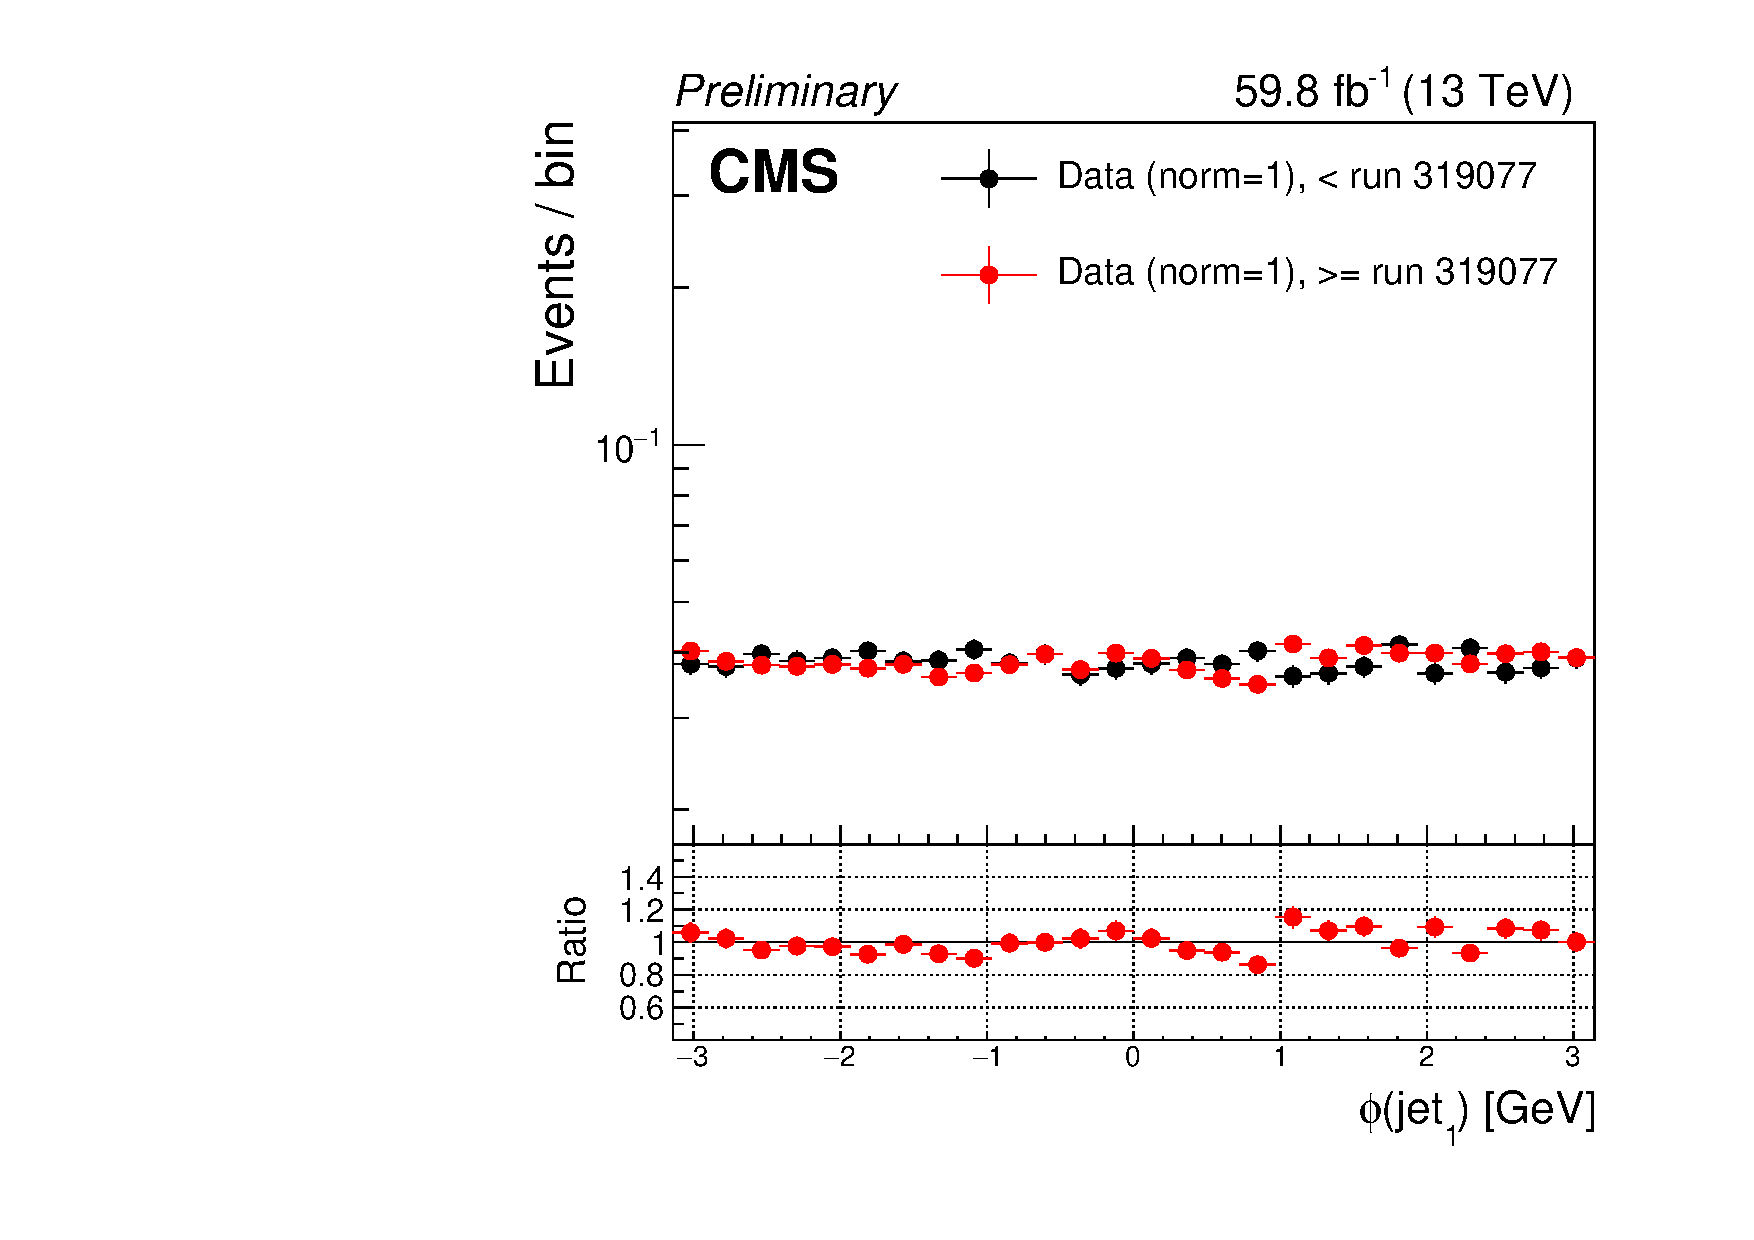
\includegraphics[width=.49\textwidth]{Images/Analysis/Results_HEMFailureStudyPlots_Data_BeforeAfterRun319077/BasicLQ_uujj_Phi_jet1_standard.pdf}}
    {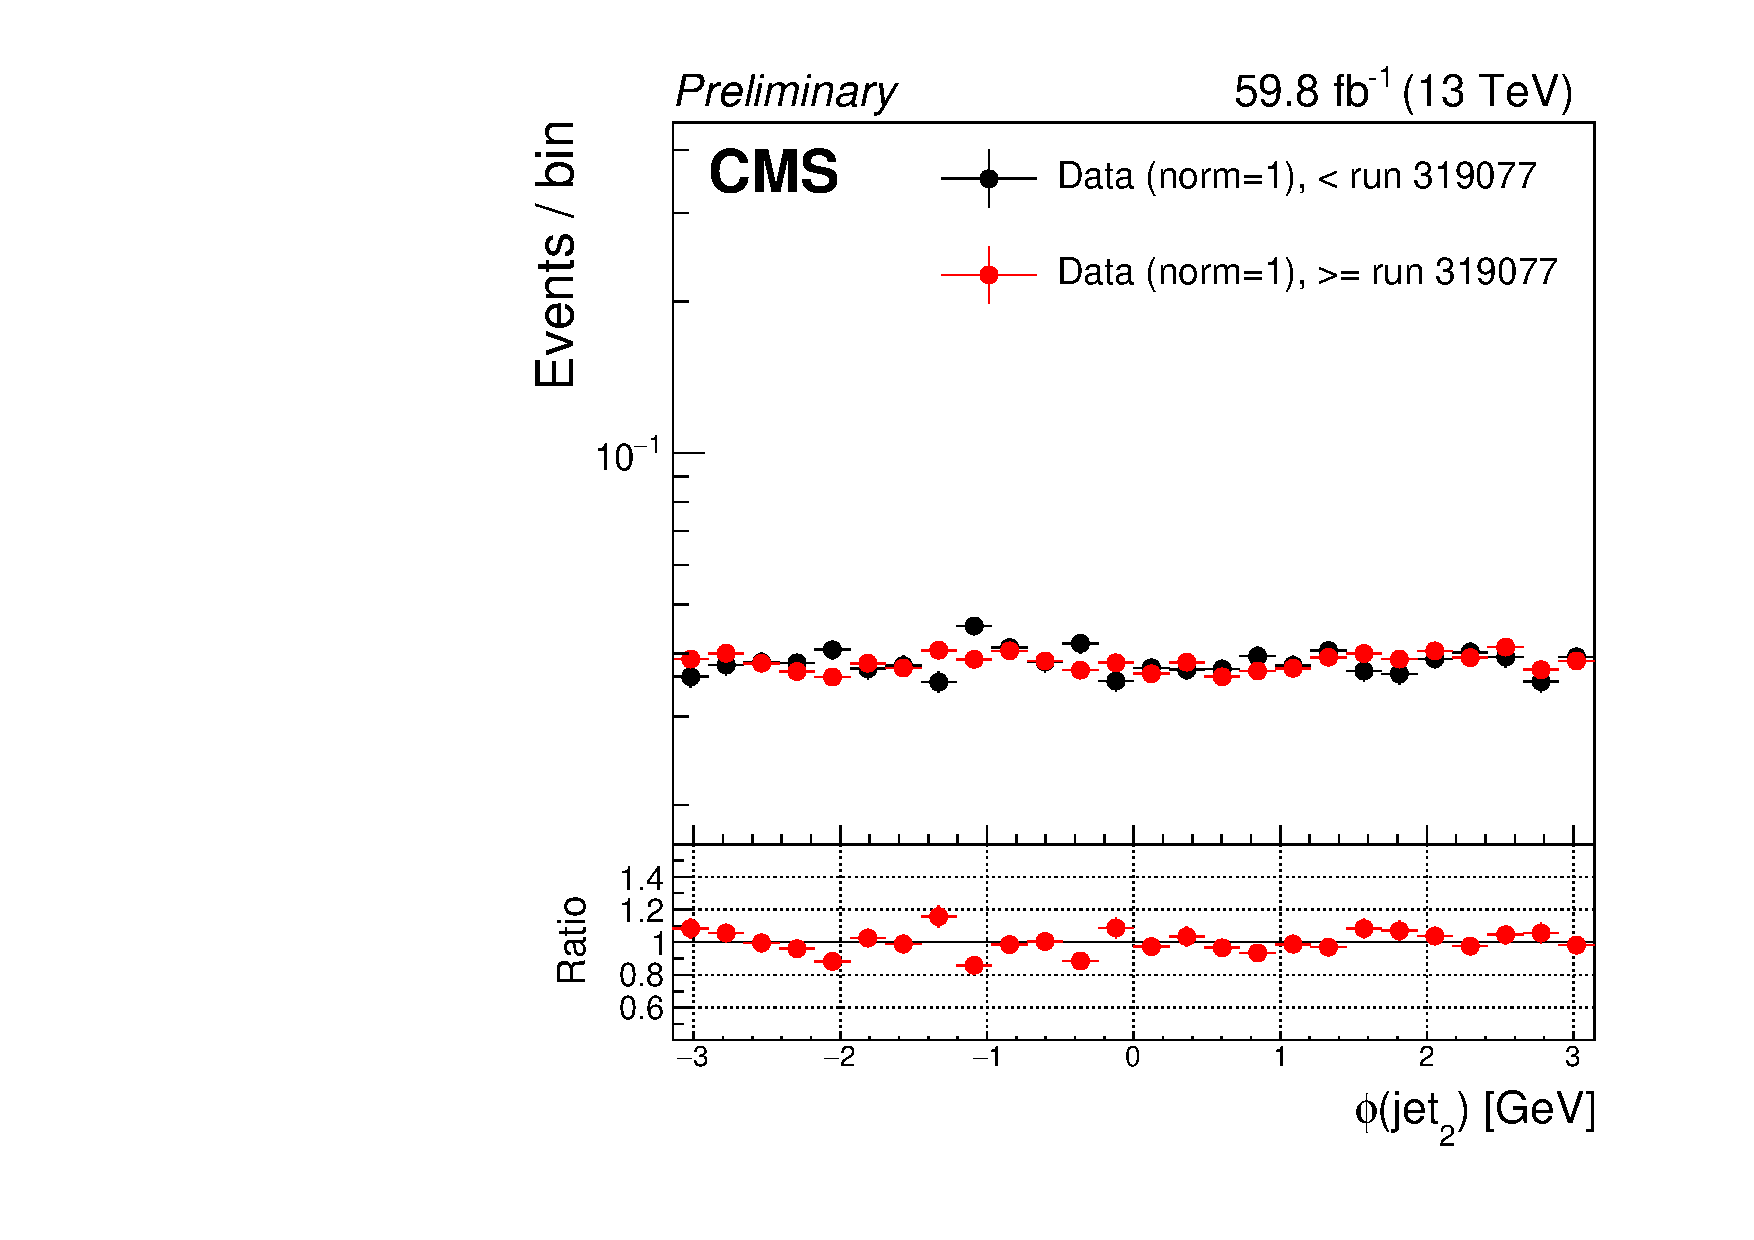
\includegraphics[width=.49\textwidth]{Images/Analysis/Results_HEMFailureStudyPlots_Data_BeforeAfterRun319077/BasicLQ_uujj_Phi_jet2_standard.pdf}}
    {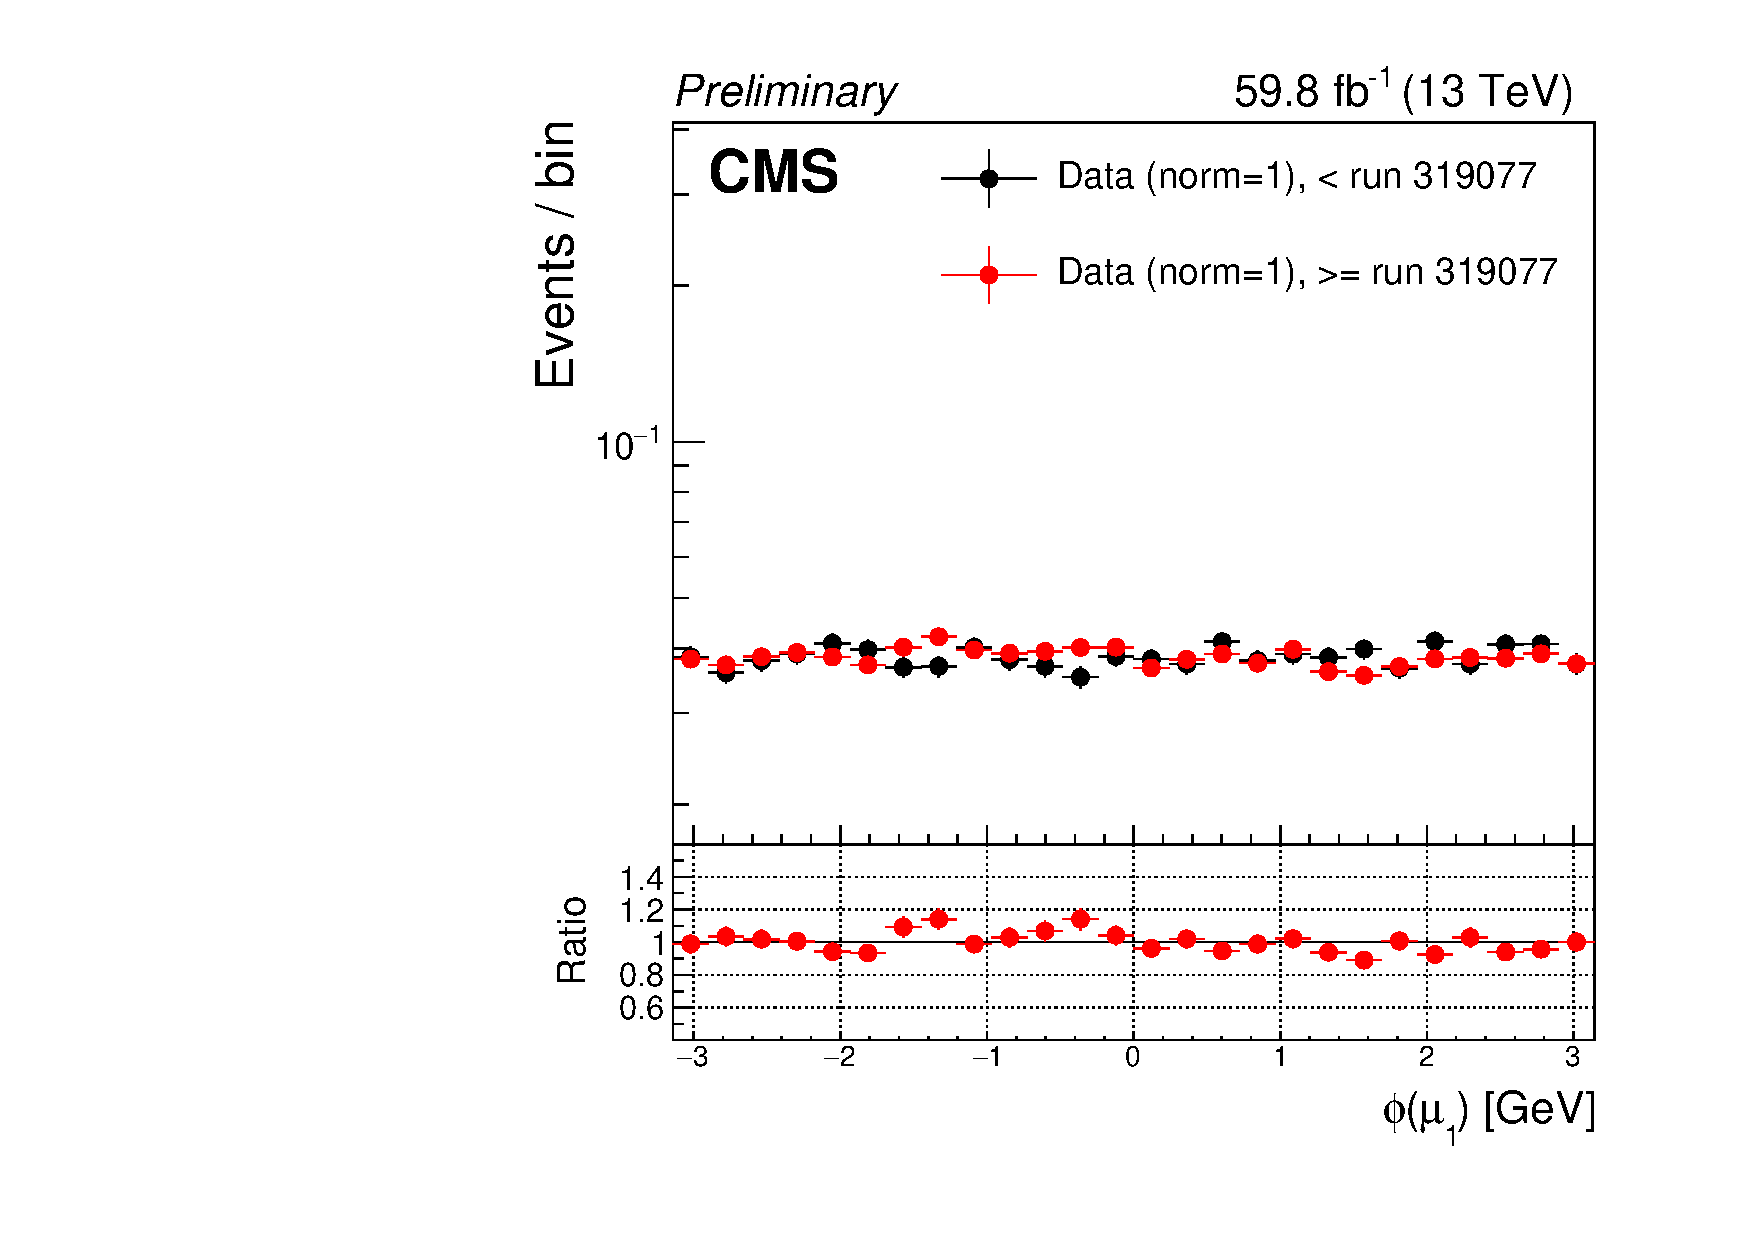
\includegraphics[width=.49\textwidth]{Images/Analysis/Results_HEMFailureStudyPlots_Data_BeforeAfterRun319077/BasicLQ_uujj_Phi_muon1_standard.pdf}}
    {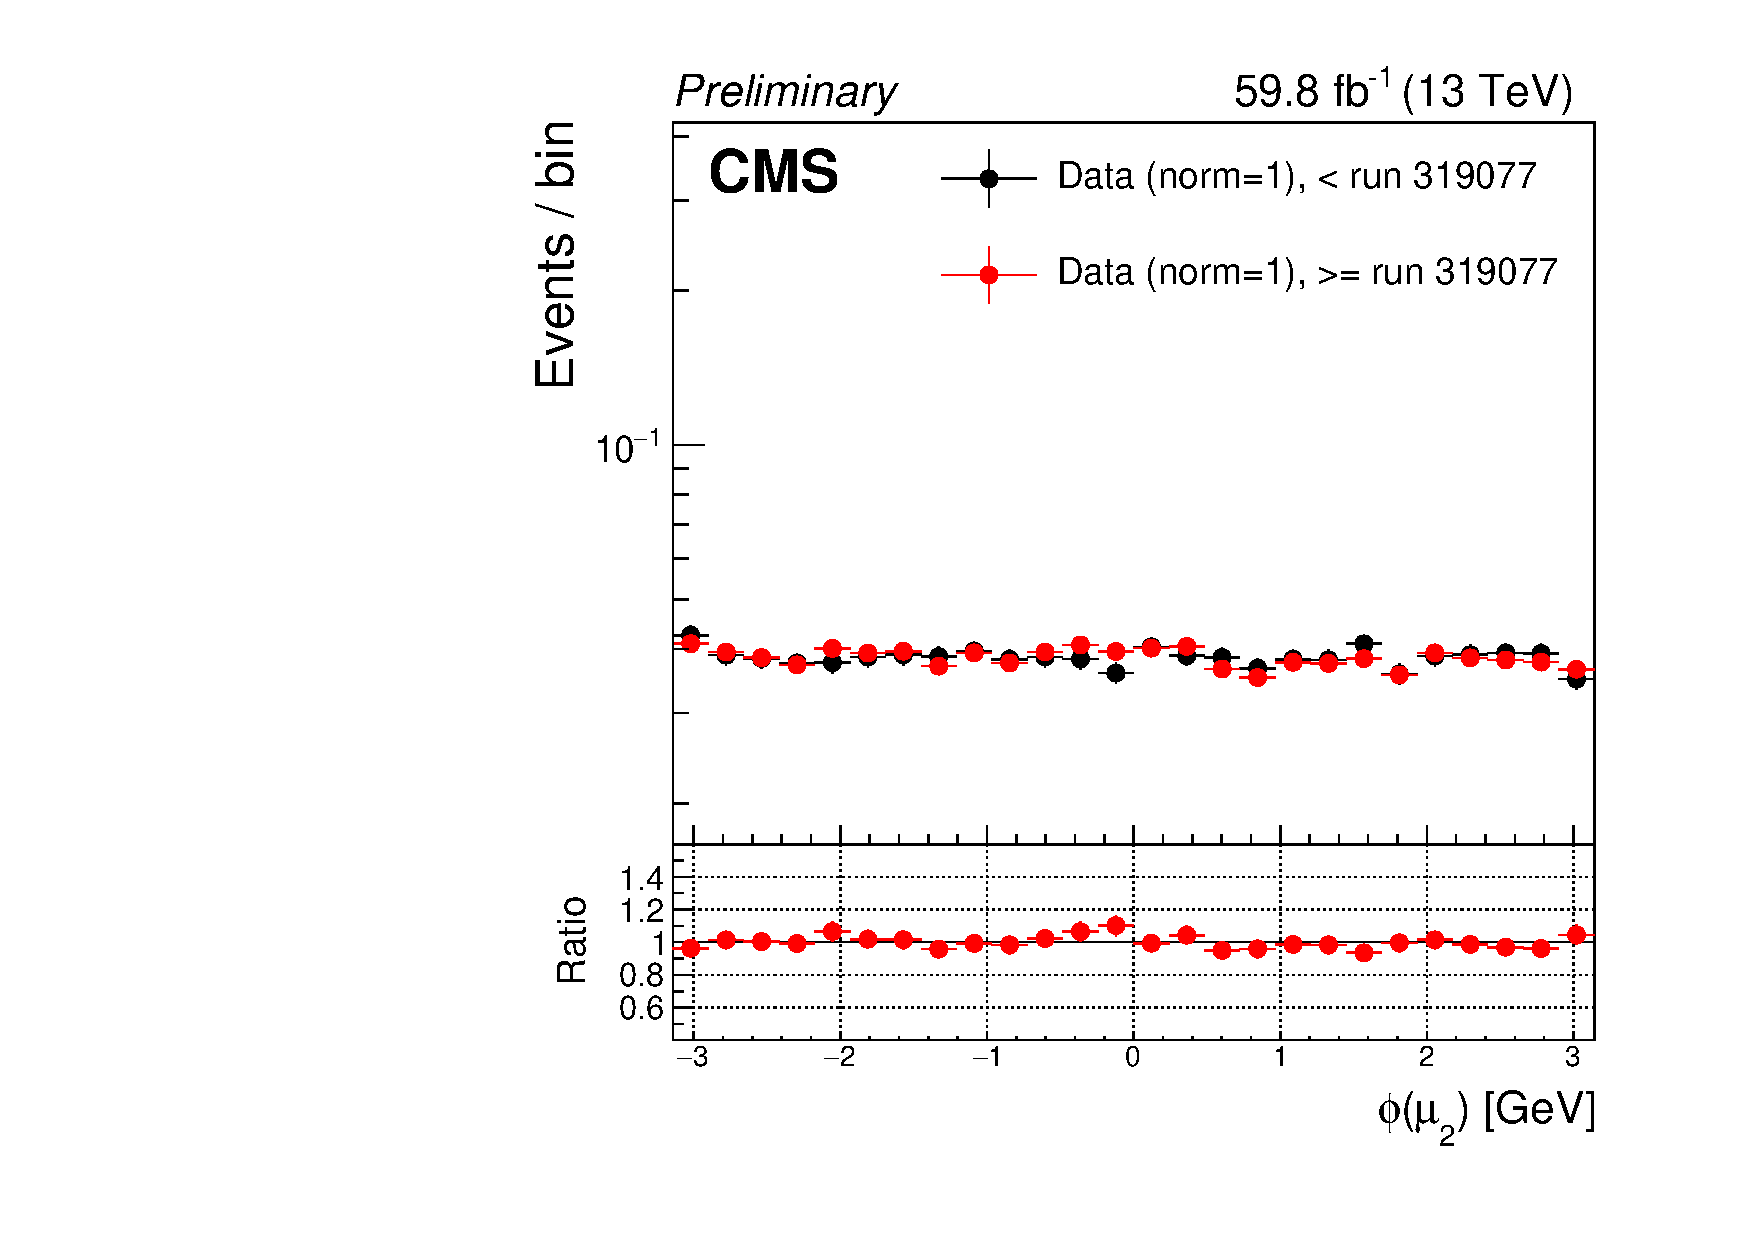
\includegraphics[width=.49\textwidth]{Images/Analysis/Results_HEMFailureStudyPlots_Data_BeforeAfterRun319077/BasicLQ_uujj_Phi_muon2_standard.pdf}}
    \caption{A shape comparison of 2018 data in periods A (black) and B (red). Data in each period have been normalized to unity and have preselection applied. The ratio \RatioDataAB is shown in the subplot. Vertical error bars represent the statistical uncertainty in each bin.}
    \label{figapp:hemjetmuonphi}
\end{figure}

\begin{figure}[H]
    \centering
    {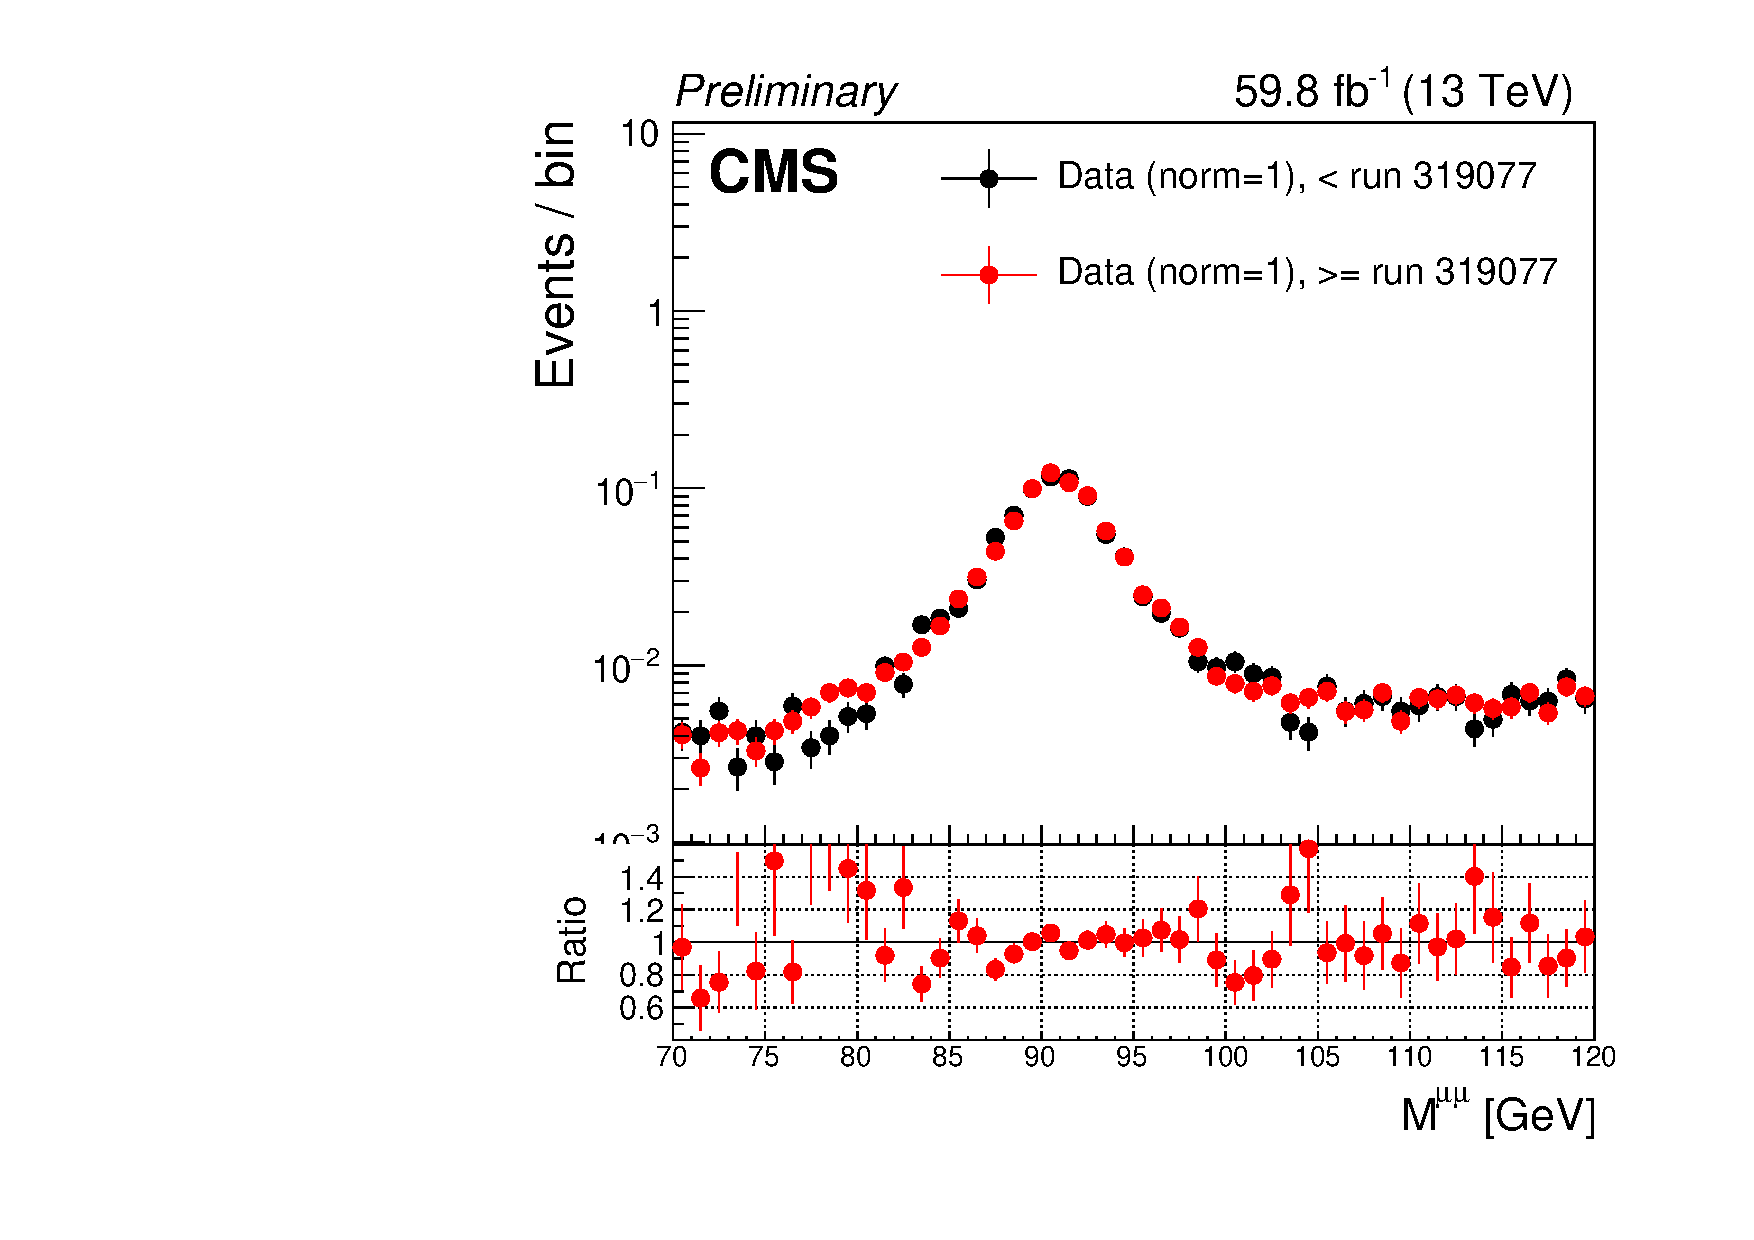
\includegraphics[width=.49\textwidth]{Images/Analysis/Results_HEMFailureStudyPlots_Data_BeforeAfterRun319077/BasicLQ_uujj_M_uu_controlzoom_ZRegion.pdf}}
    {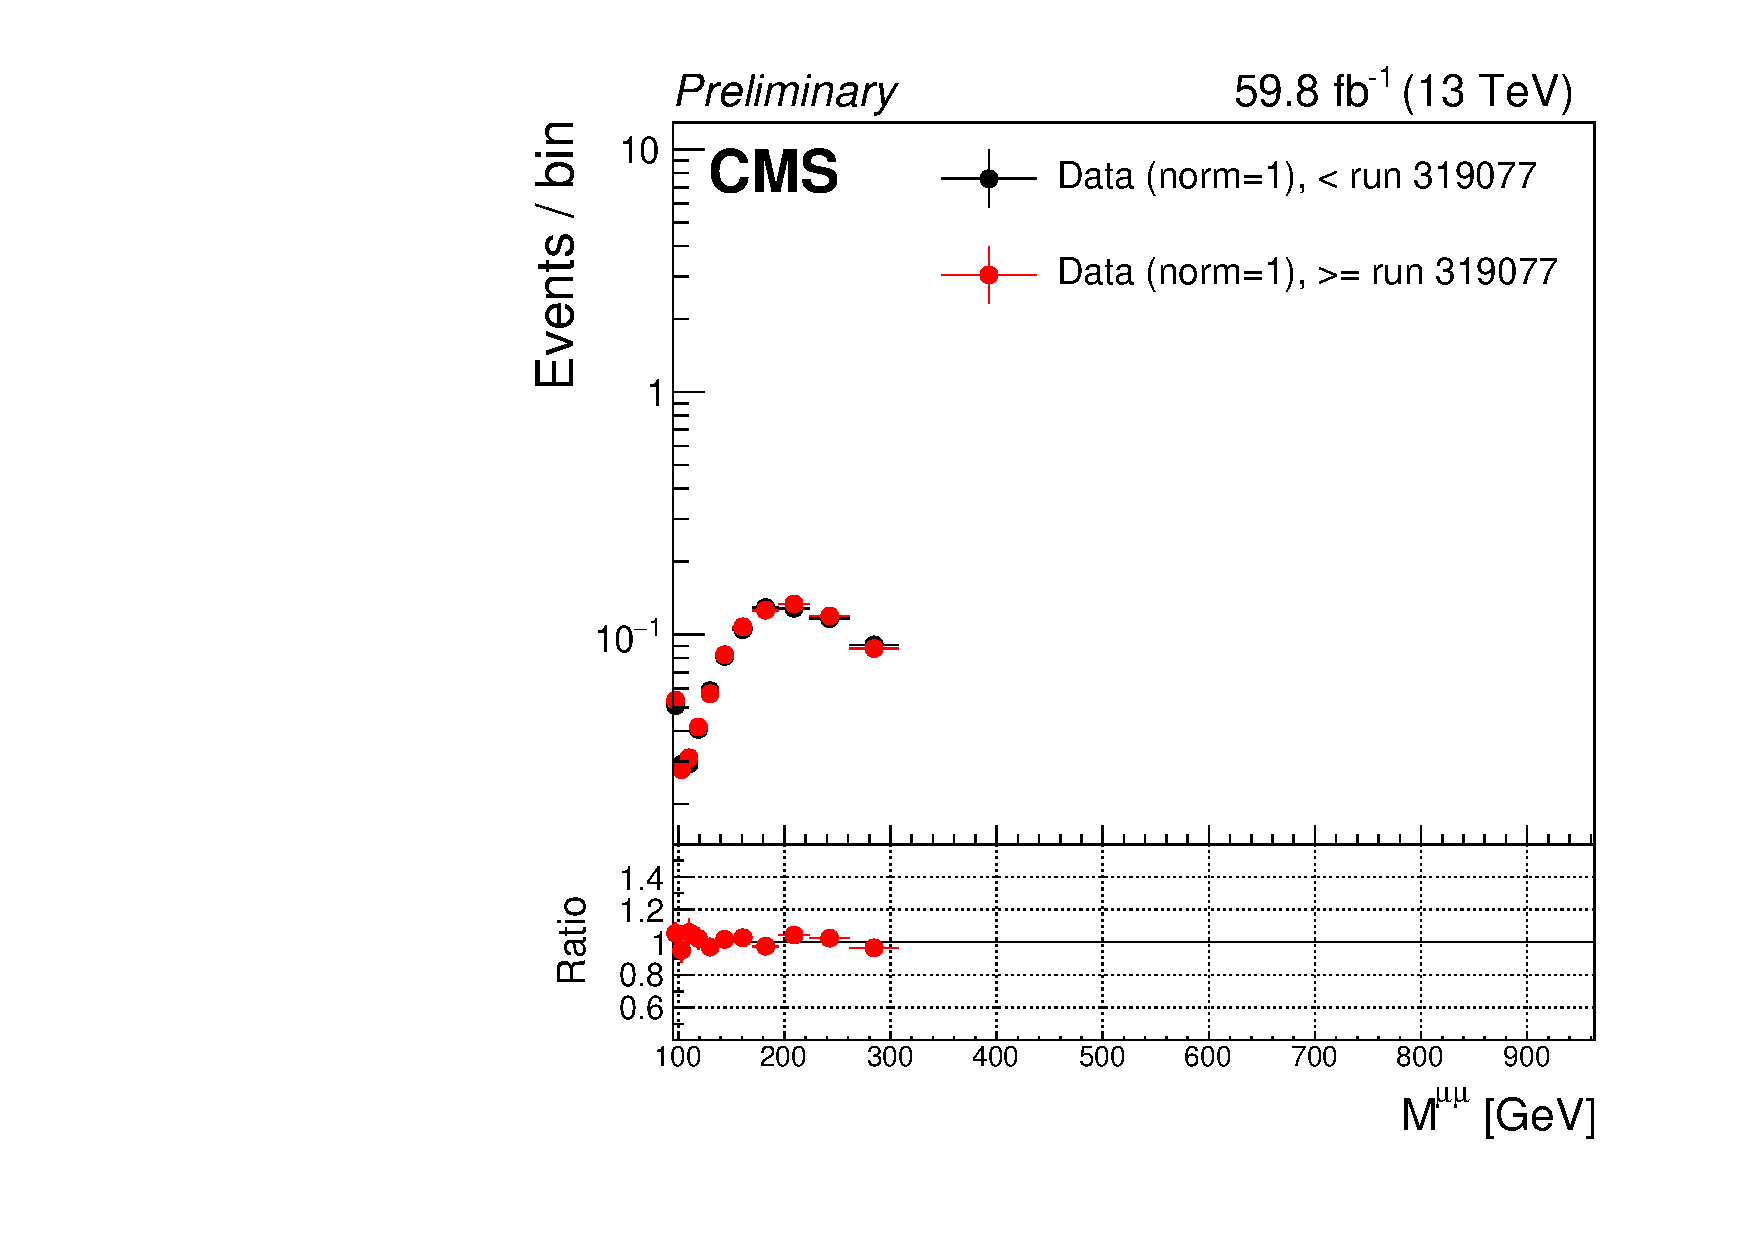
\includegraphics[width=.49\textwidth]{Images/Analysis/Results_HEMFailureStudyPlots_Data_BeforeAfterRun319077/BasicLQ_uujj_M_uu_controlzoom_TTRegion.pdf}}
    \caption{A shape comparison of 2018 data in periods A (black) and B (red). Data in each period have been normalized to unity and have preselection applied. The ratio \RatioDataAB is shown in the subplot. Vertical error bars represent the statistical uncertainty in each bin.}
    \label{figapp:hemMuuZoom}
\end{figure}

\begin{figure}[H]
    \centering
    {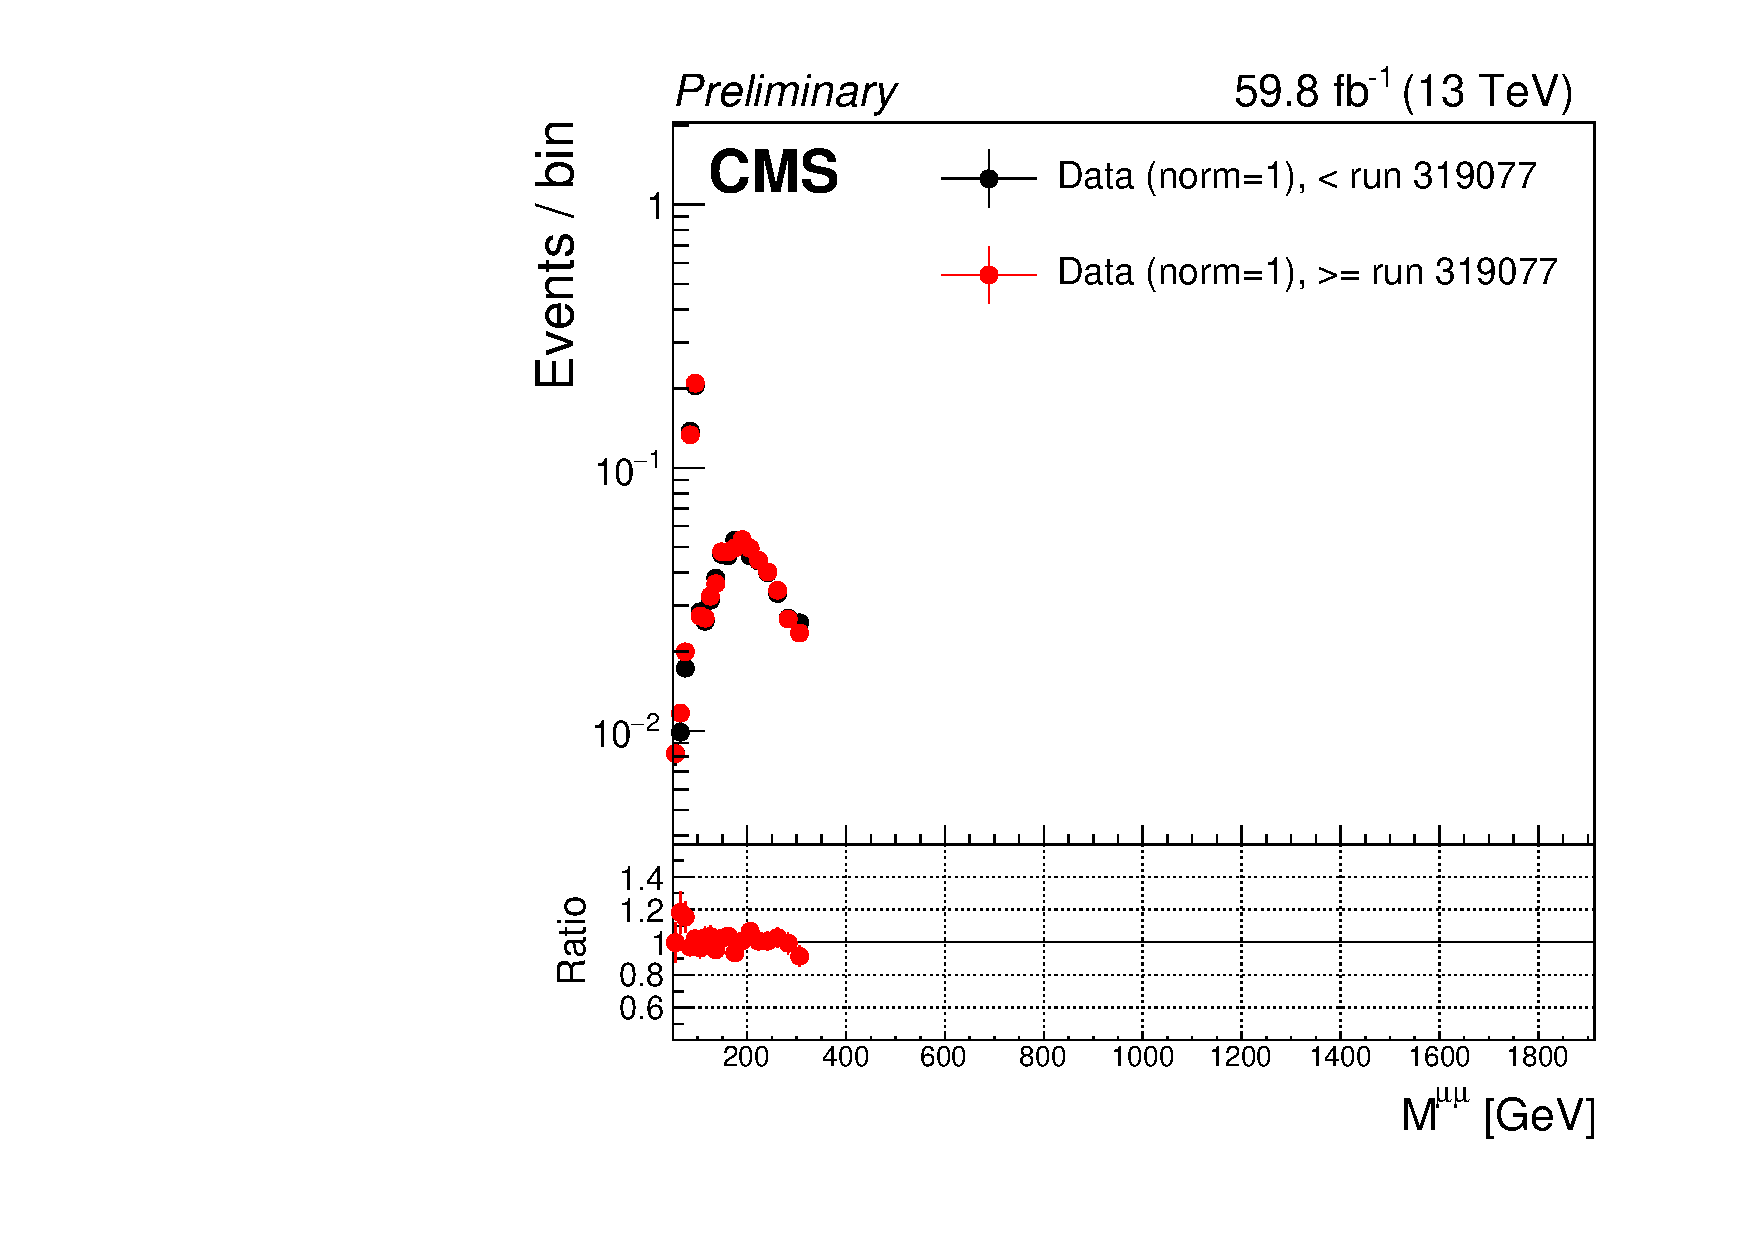
\includegraphics[width=.49\textwidth]{Images/Analysis/Results_HEMFailureStudyPlots_Data_BeforeAfterRun319077/BasicLQ_uujj_M_uu_standard.pdf}}
    {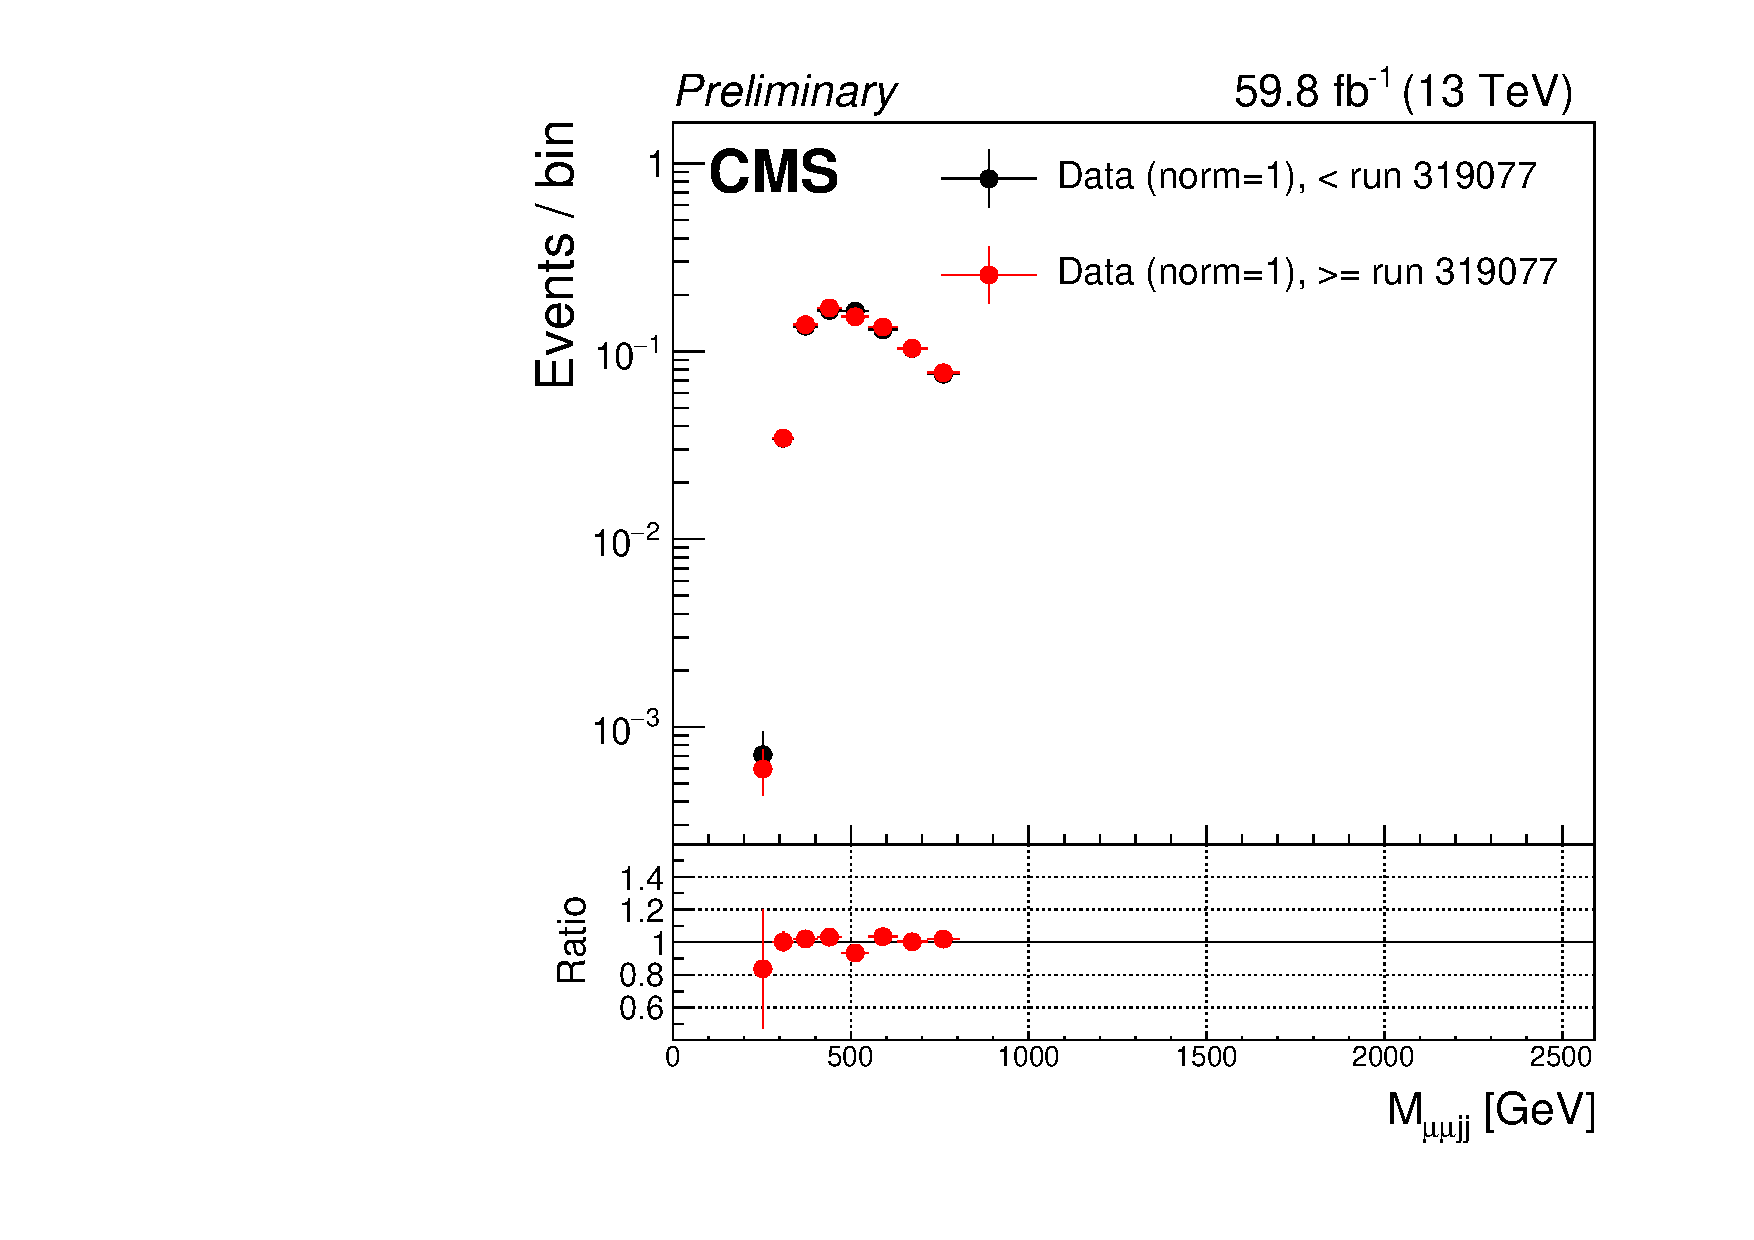
\includegraphics[width=.49\textwidth]{Images/Analysis/Results_HEMFailureStudyPlots_Data_BeforeAfterRun319077/BasicLQ_uujj_M_uujj_standard.pdf}}
    {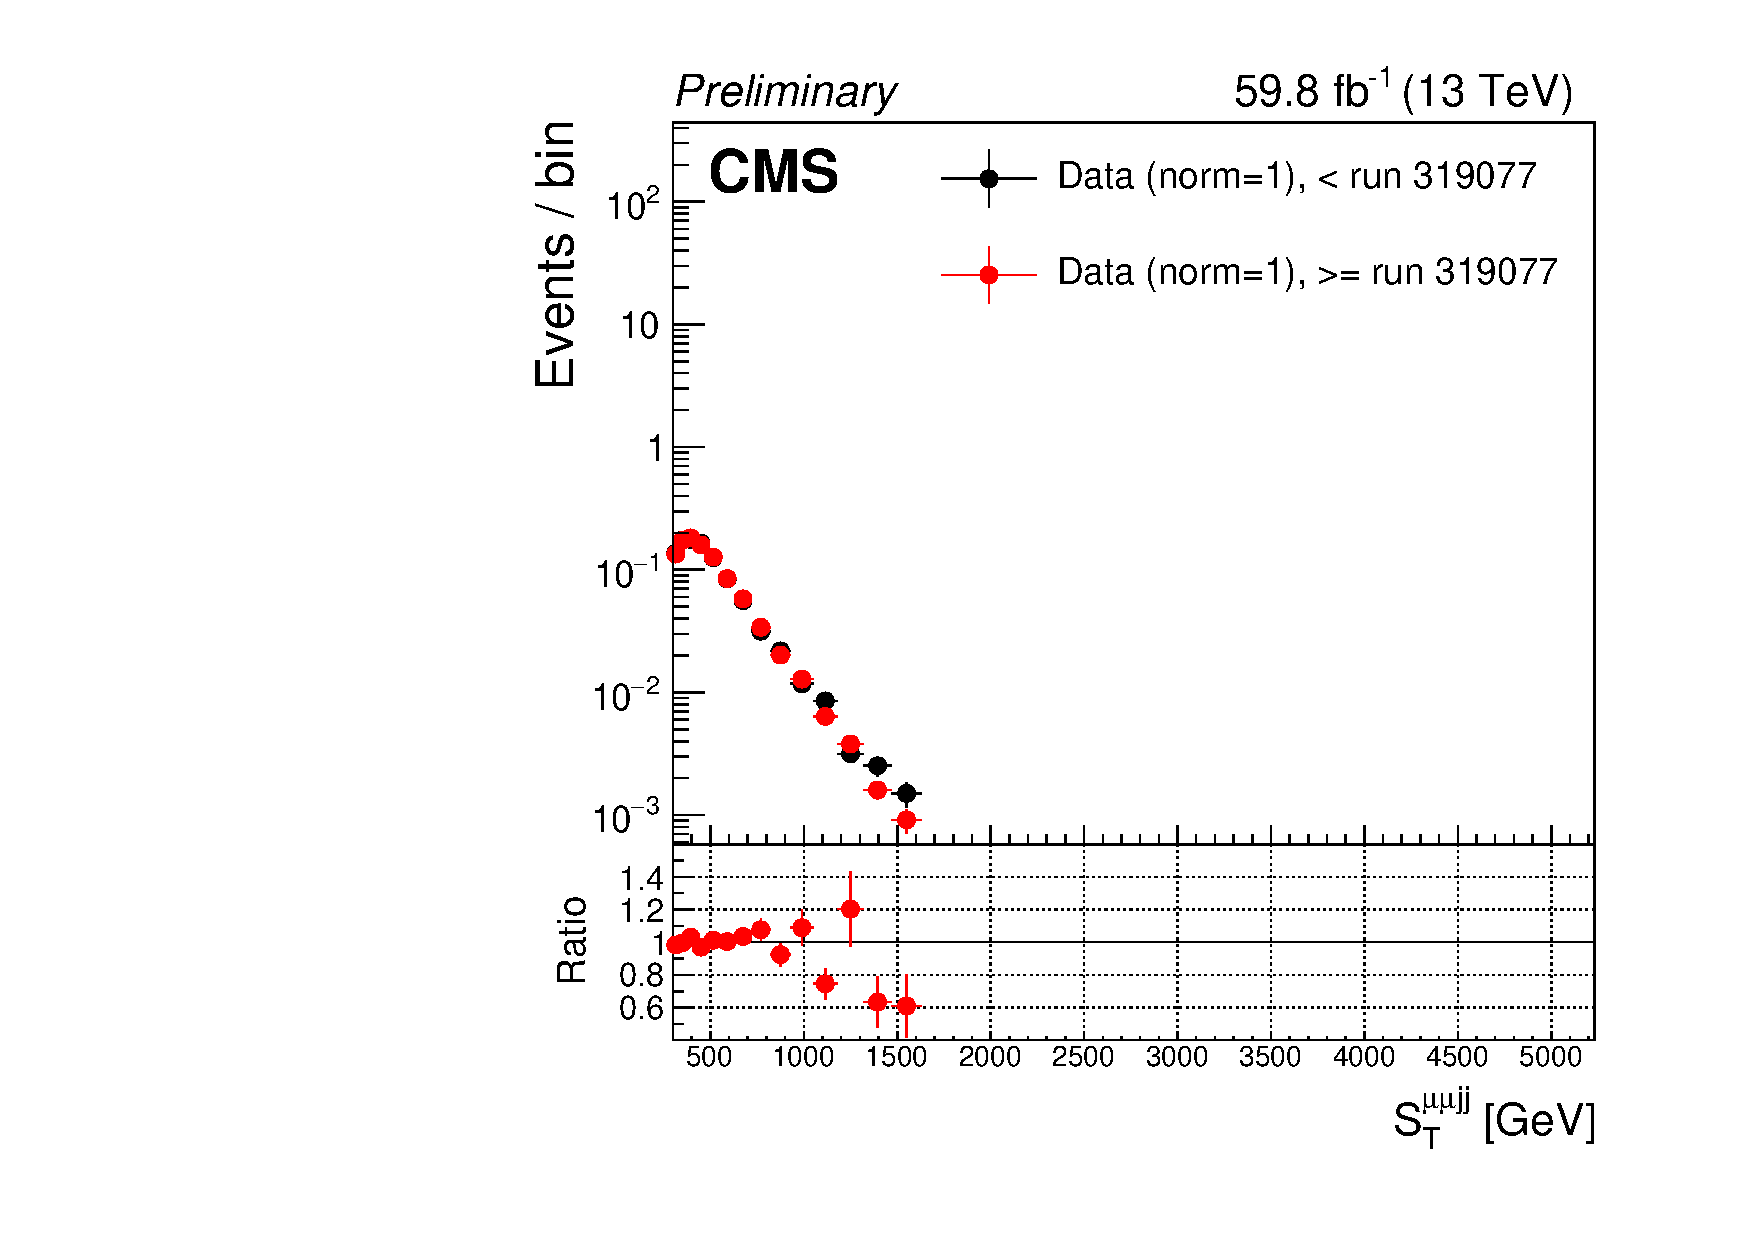
\includegraphics[width=.49\textwidth]{Images/Analysis/Results_HEMFailureStudyPlots_Data_BeforeAfterRun319077/BasicLQ_uujj_St_uujj_standard.pdf}}
    \caption{A shape comparison of 2018 data in periods A (black) and B (red). Data in each period have been normalized to unity and have preselection applied. The ratio \RatioDataAB is shown in the subplot. Vertical error bars represent the statistical uncertainty in each bin.}
    \label{figapp:hemMuuMuujjSt}
\end{figure}

\begin{figure}[H]
    \centering
    {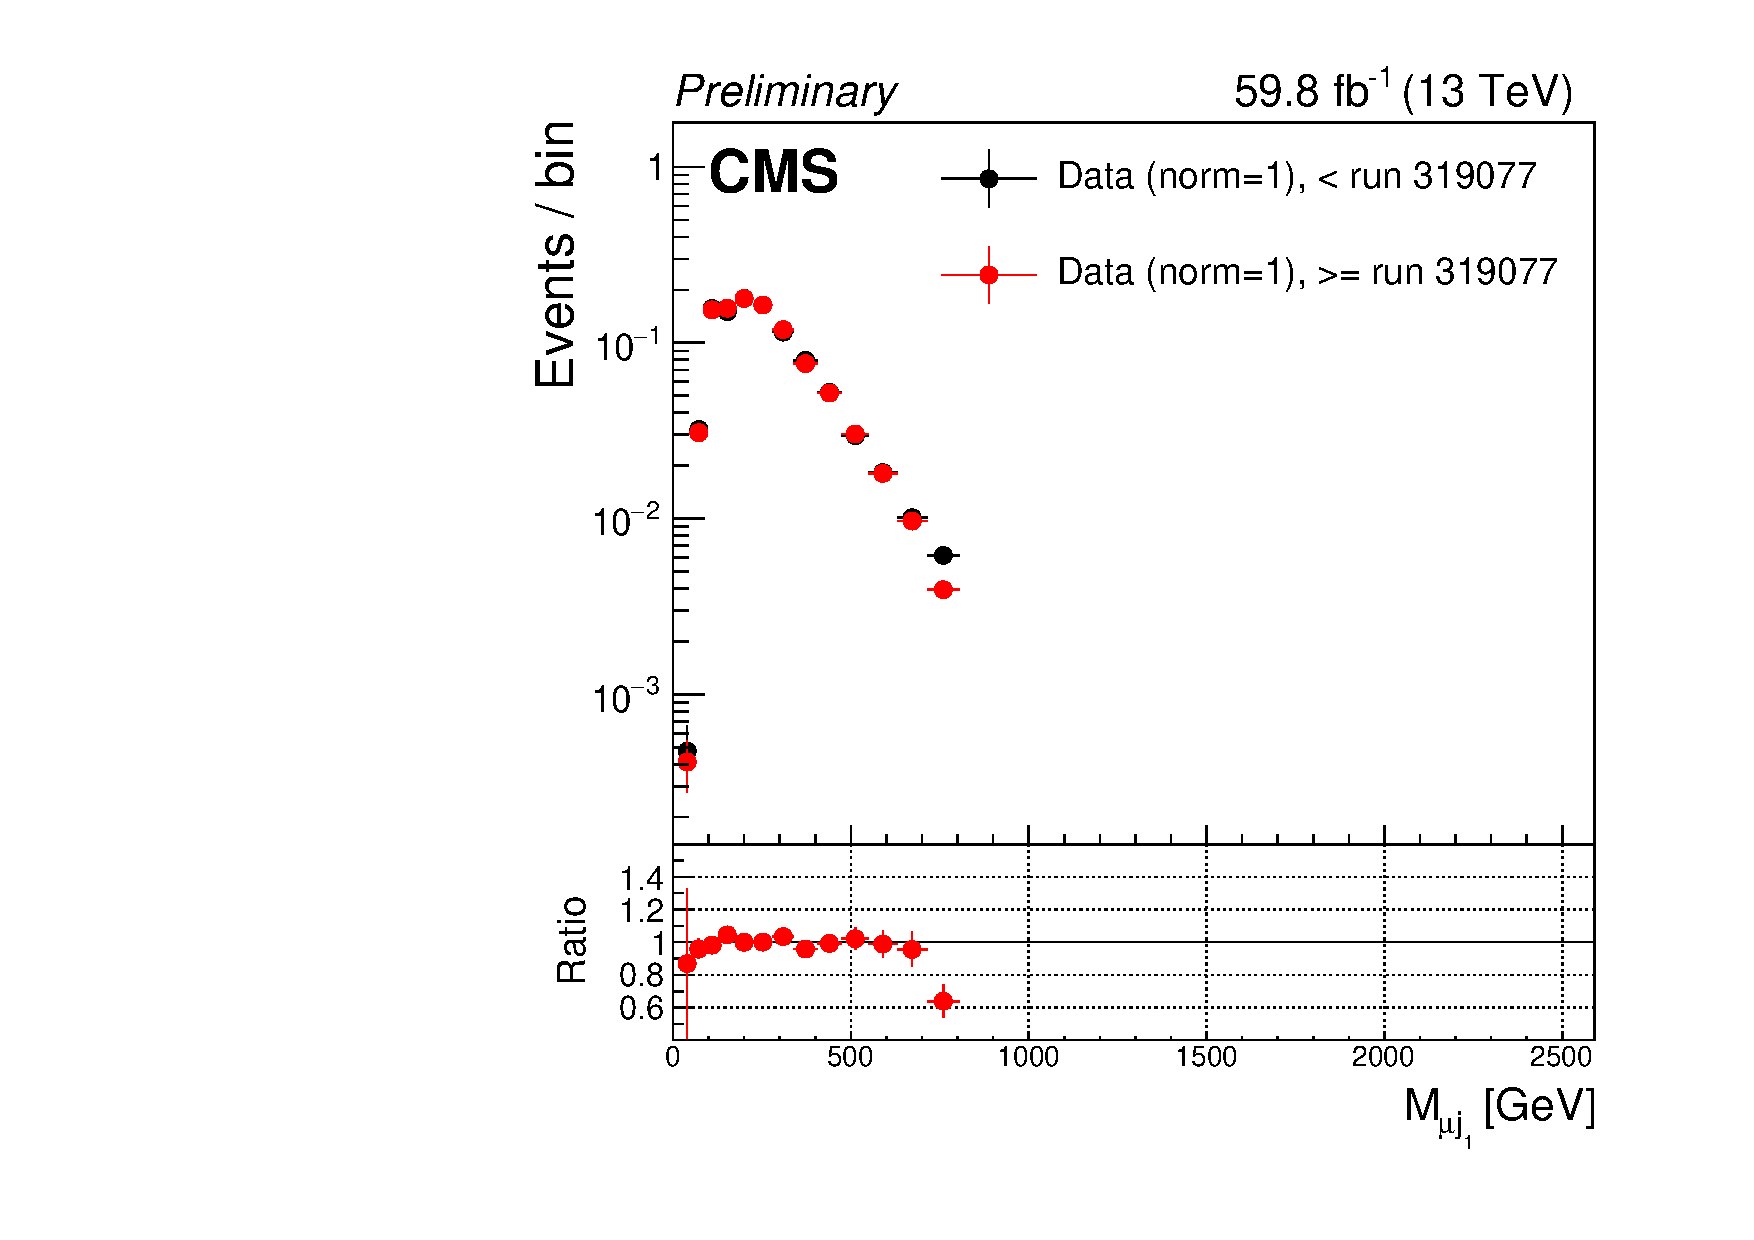
\includegraphics[width=.49\textwidth]{Images/Analysis/Results_HEMFailureStudyPlots_Data_BeforeAfterRun319077/BasicLQ_uujj_M_uujj1_standard.pdf}}
    {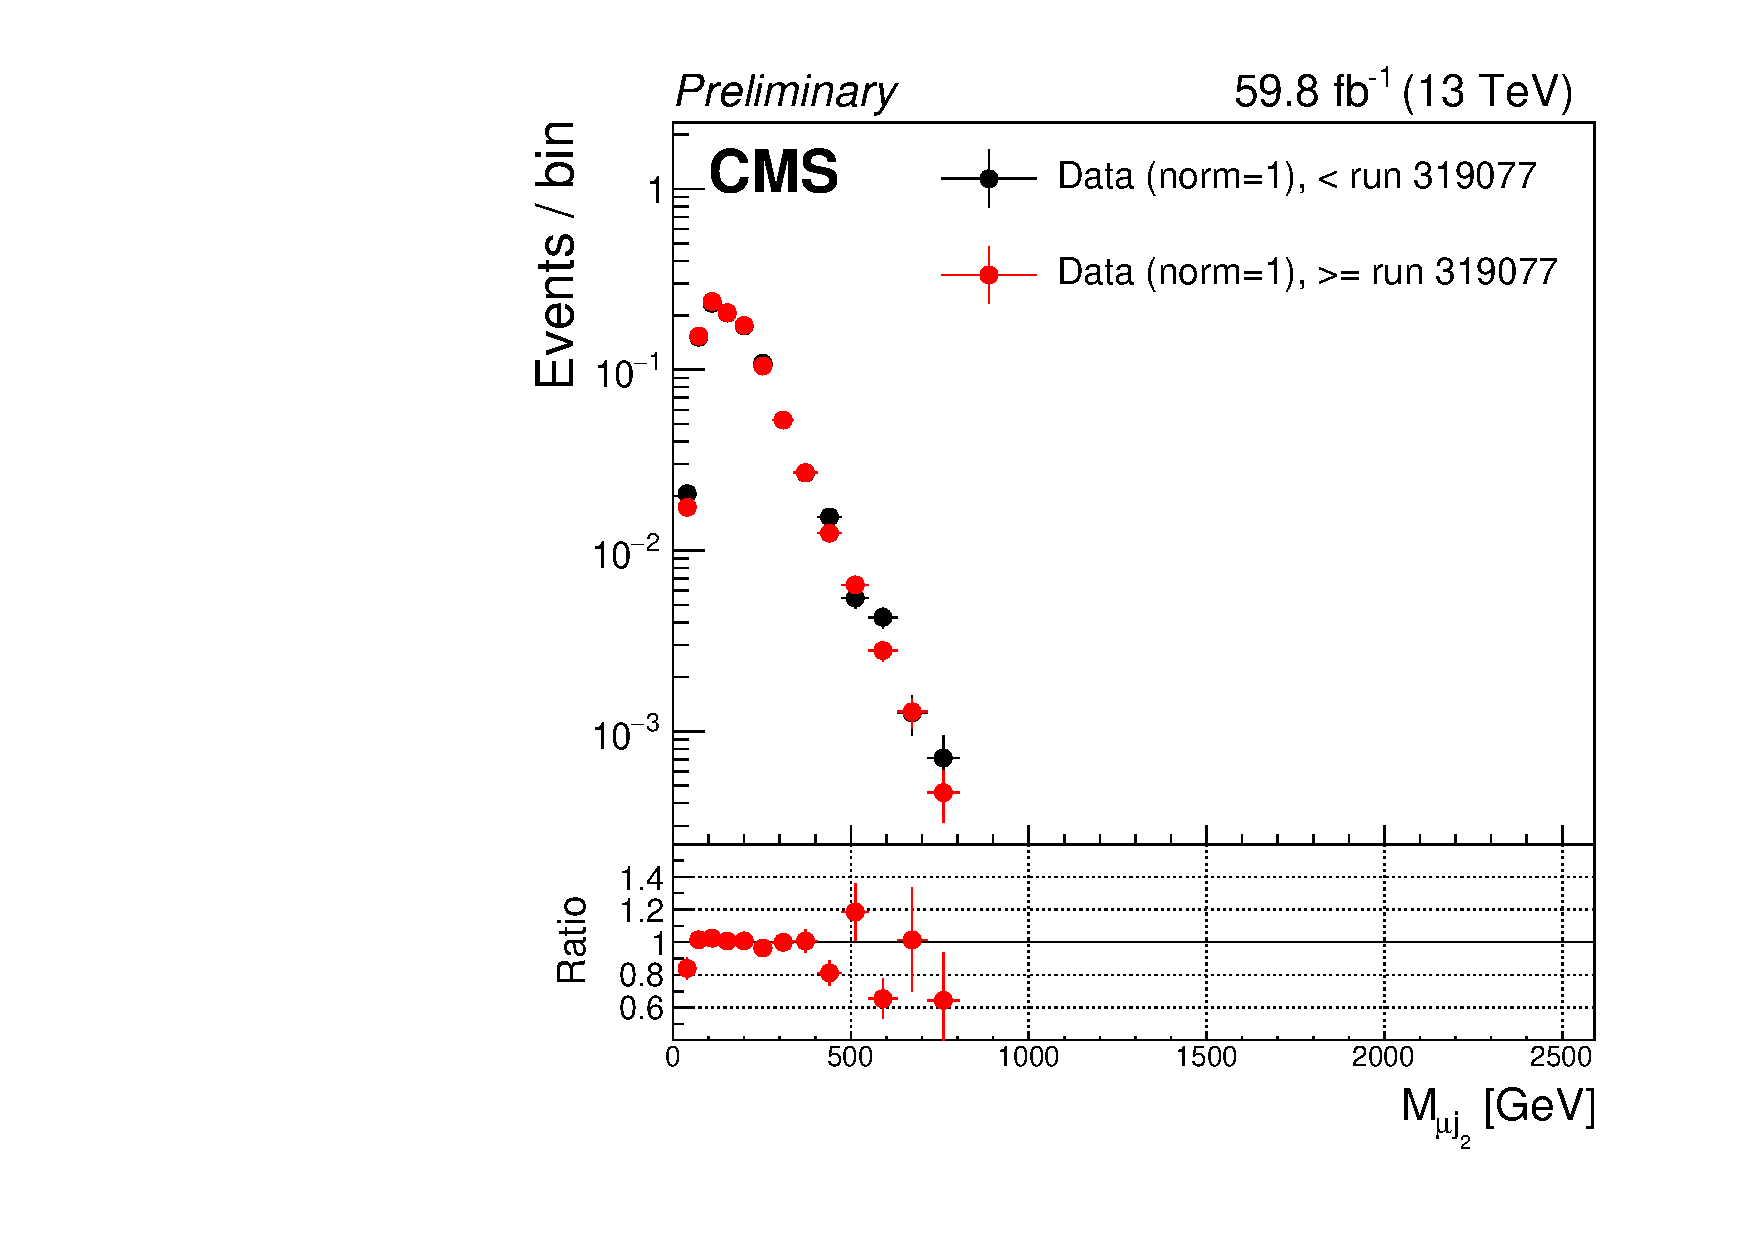
\includegraphics[width=.49\textwidth]{Images/Analysis/Results_HEMFailureStudyPlots_Data_BeforeAfterRun319077/BasicLQ_uujj_M_uujj2_standard.pdf}}
    \caption{A shape comparison of 2018 data in periods A (black) and B (red). Data in each period have been normalized to unity and have preselection applied. The ratio \RatioDataAB is shown in the subplot. Vertical error bars represent the statistical uncertainty in each bin.}
    \label{figapp:hemLQcandidates}
\end{figure}

\begin{figure}[H]
    \centering
    {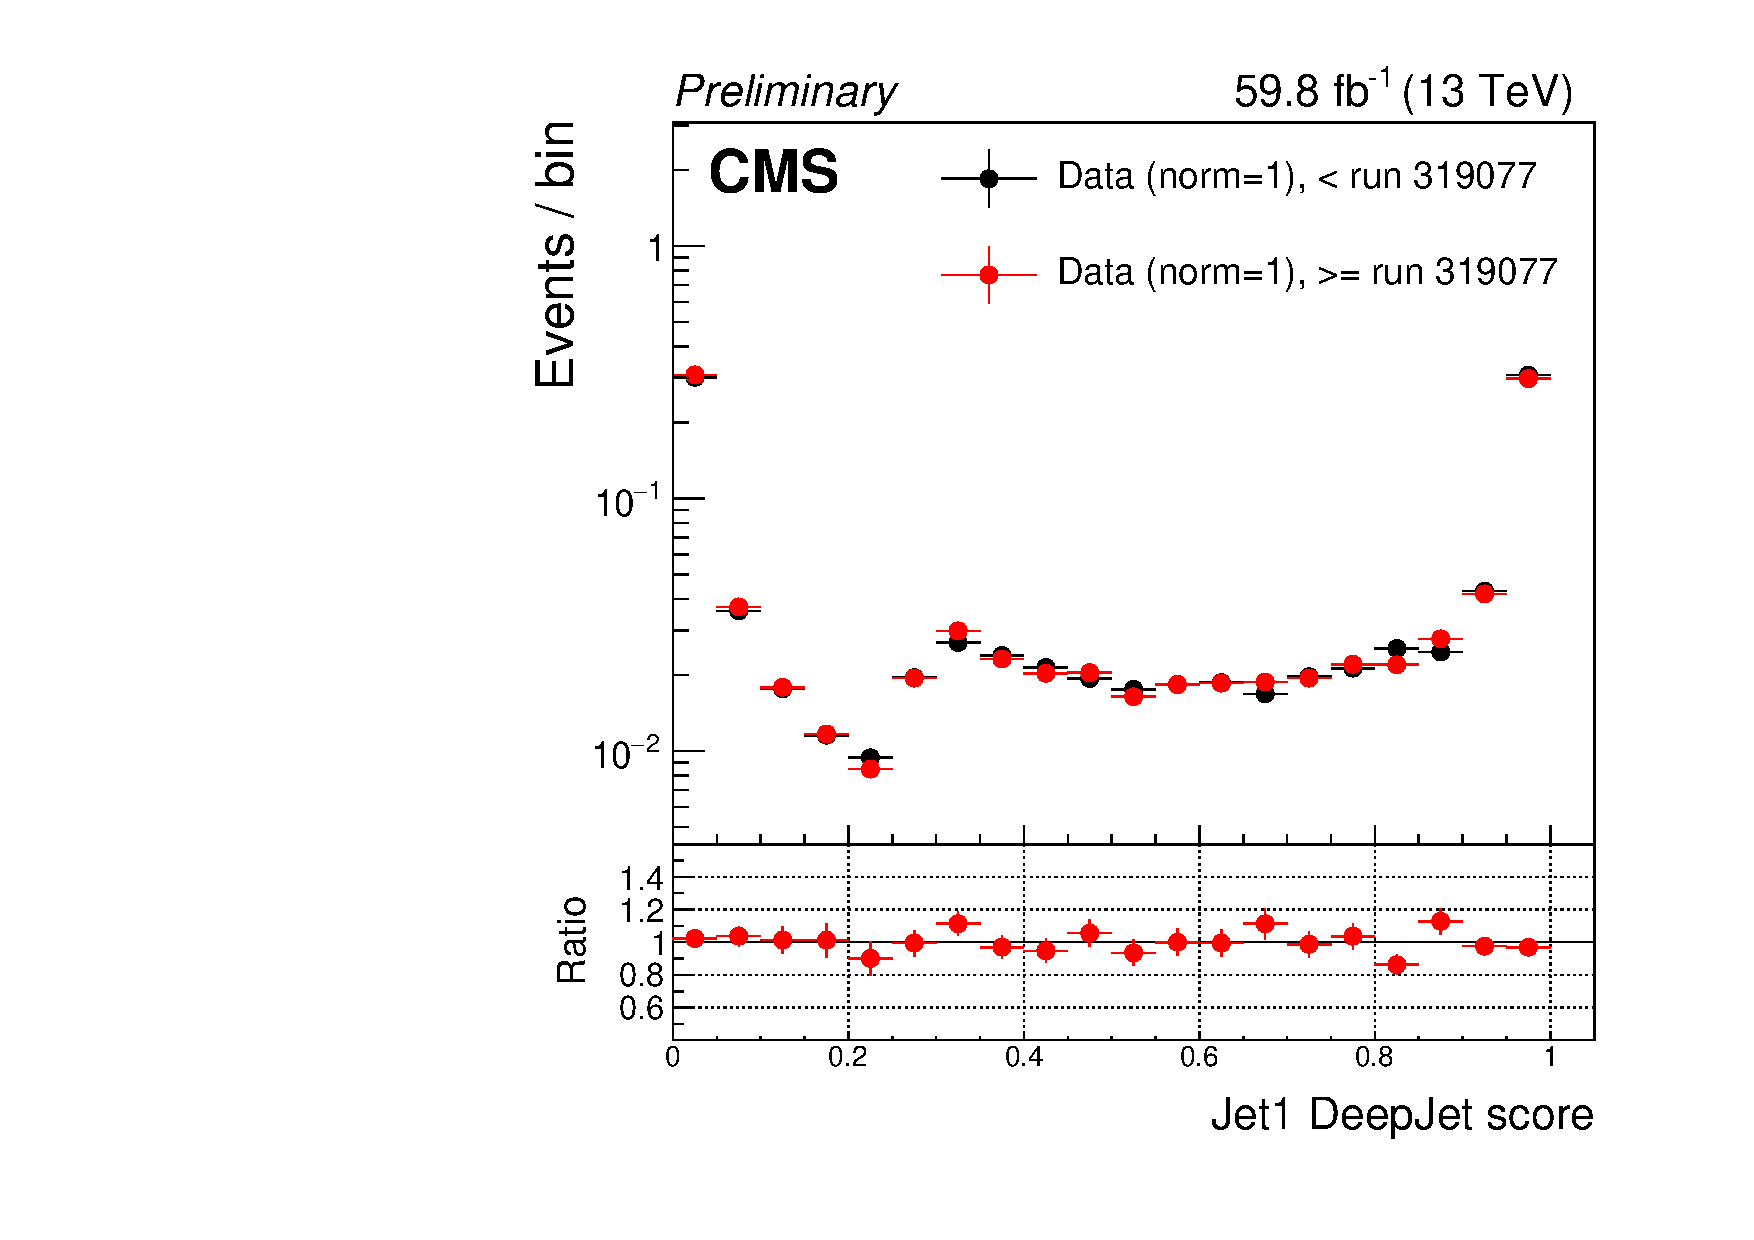
\includegraphics[width=.49\textwidth]{Images/Analysis/Results_HEMFailureStudyPlots_Data_BeforeAfterRun319077/BasicLQ_uujj_DeepJet_jet1_standard.pdf}}
    {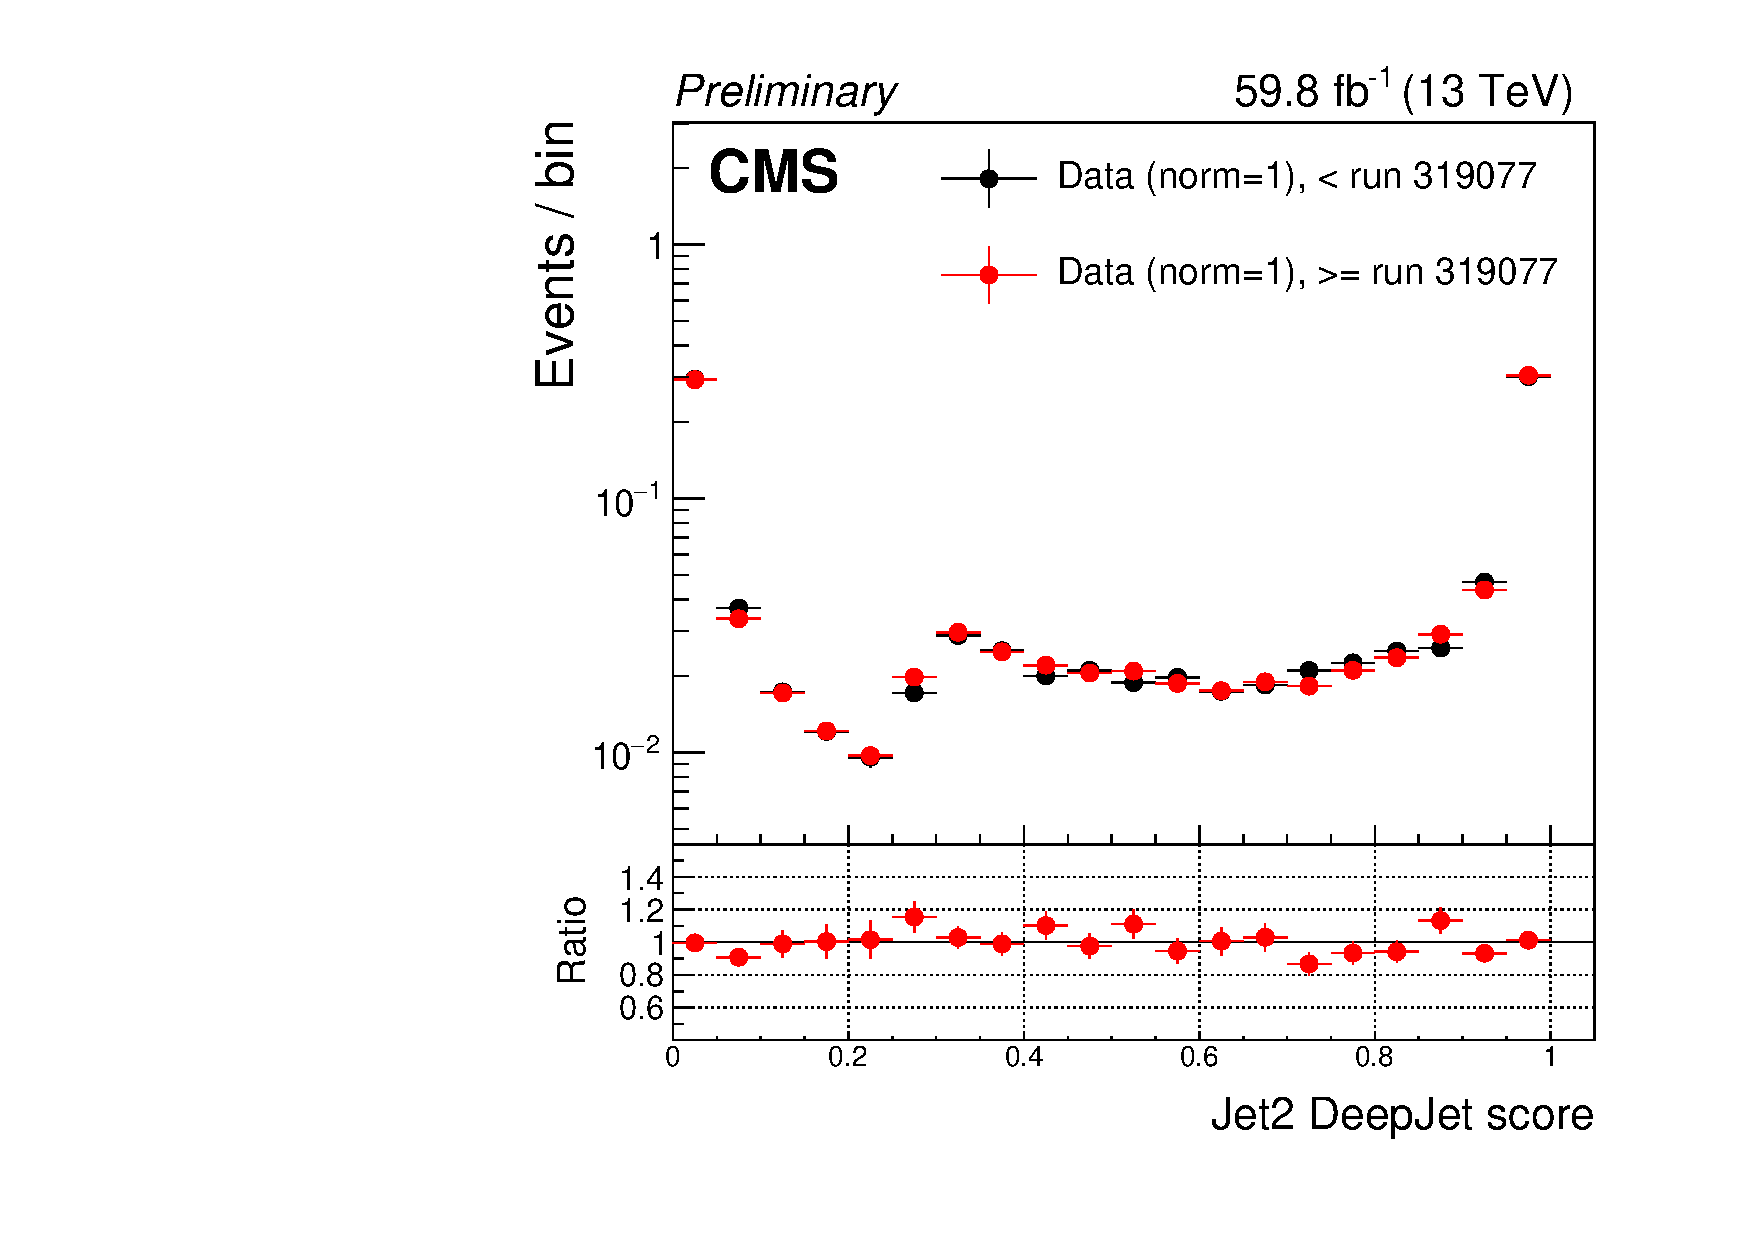
\includegraphics[width=.49\textwidth]{Images/Analysis/Results_HEMFailureStudyPlots_Data_BeforeAfterRun319077/BasicLQ_uujj_DeepJet_jet2_standard.pdf}}
    \caption{A shape comparison of 2018 data in periods A (black) and B (red). Data in each period have been normalized to unity and have preselection applied. The ratio \RatioDataAB is shown in the subplot. Vertical error bars represent the statistical uncertainty in each bin.}
    \label{figapp:hembtagscores}
\end{figure}

\begin{figure}[H]
    \centering
    {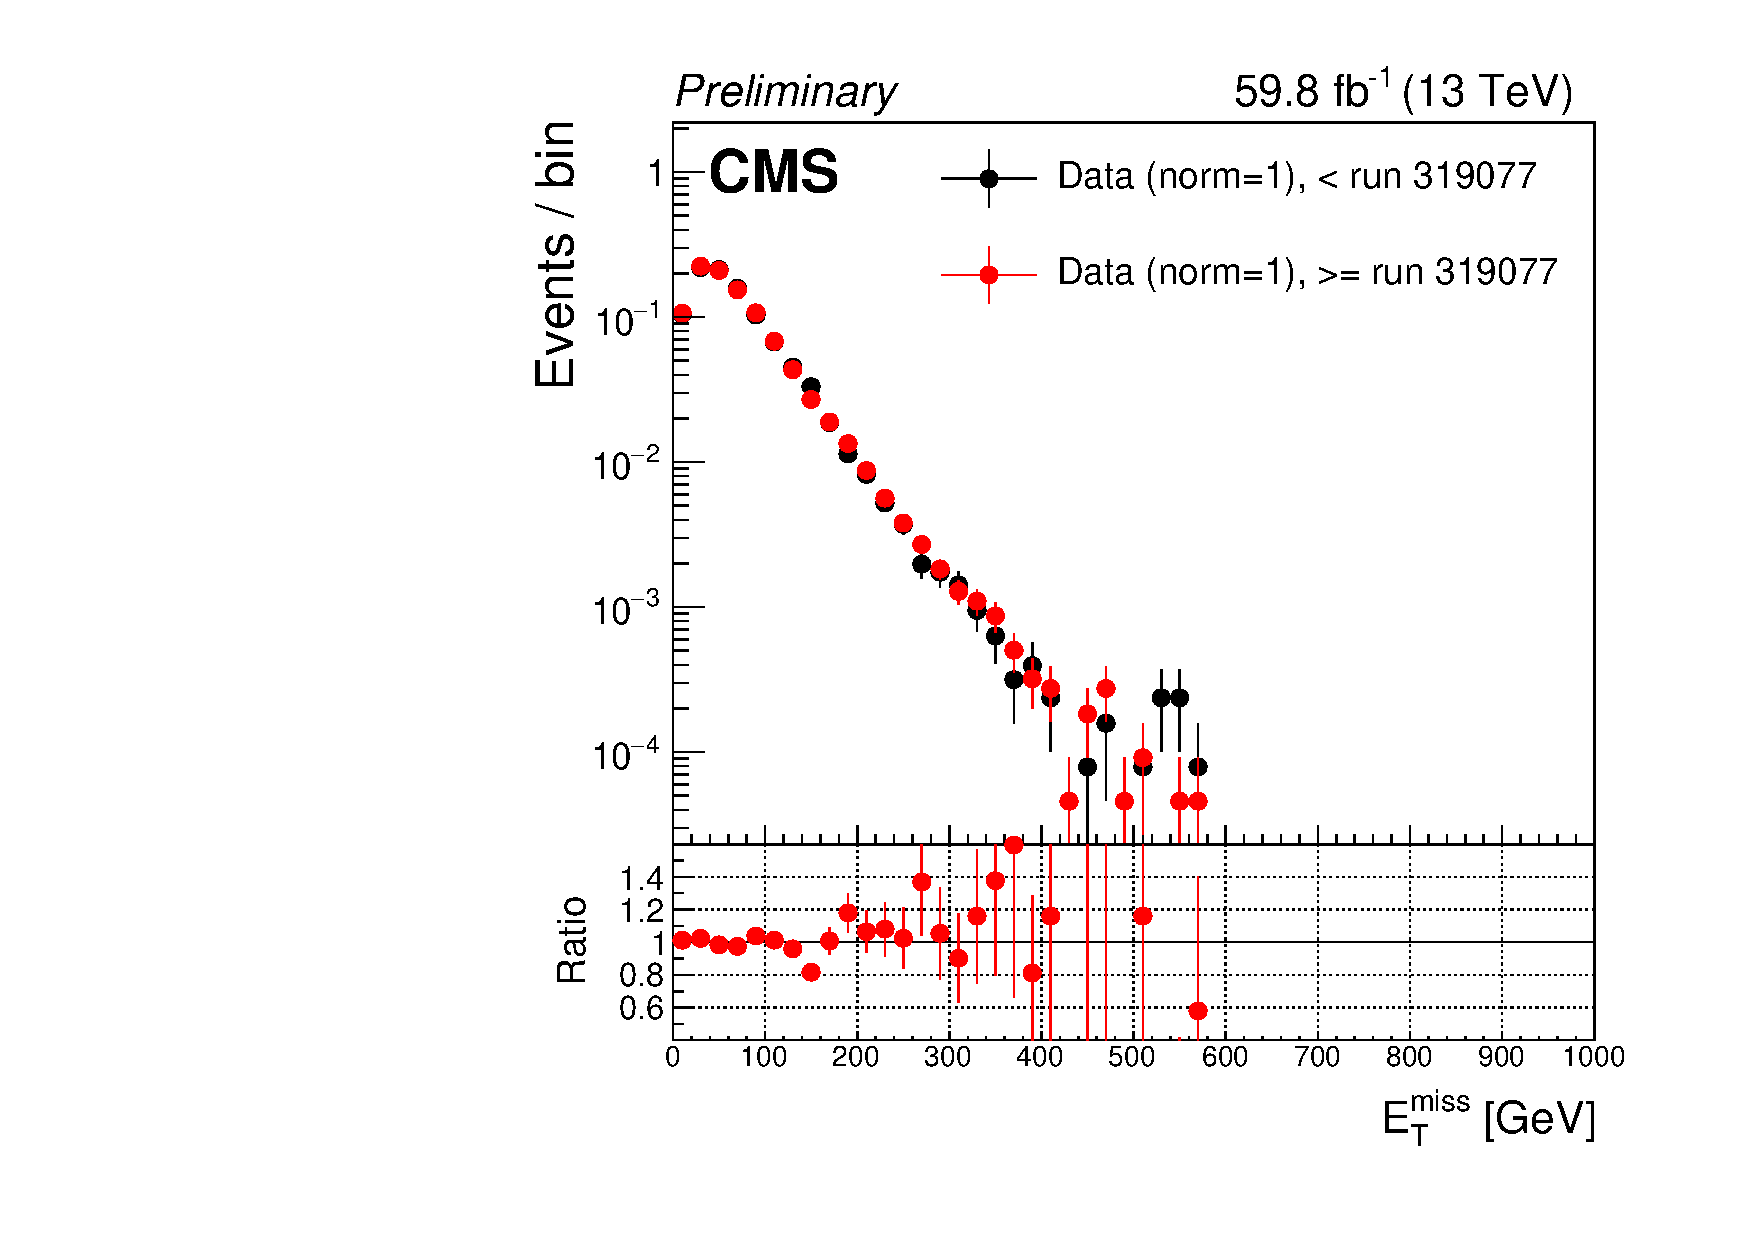
\includegraphics[width=.49\textwidth]{Images/Analysis/Results_HEMFailureStudyPlots_Data_BeforeAfterRun319077/BasicLQ_uujj_Pt_miss_standard.pdf}}
    {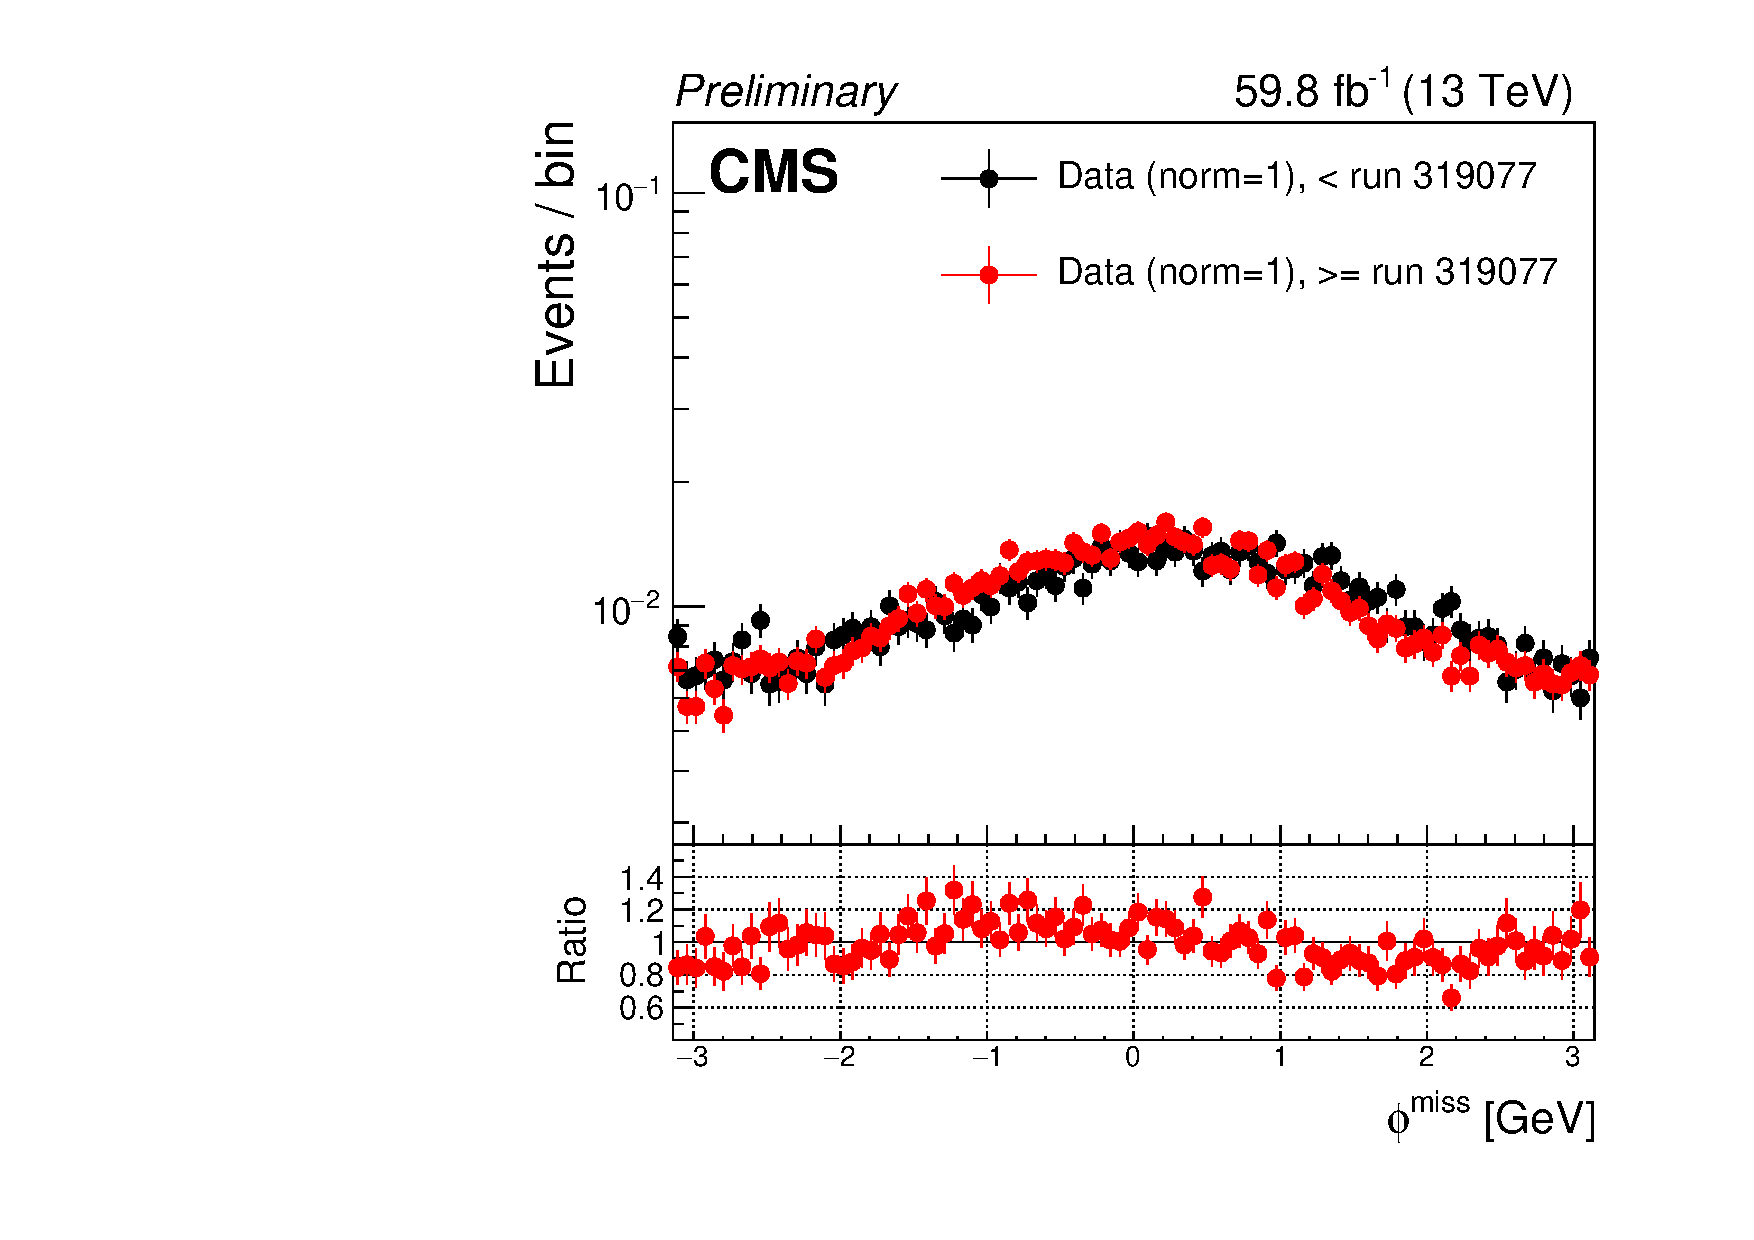
\includegraphics[width=.49\textwidth]{Images/Analysis/Results_HEMFailureStudyPlots_Data_BeforeAfterRun319077/BasicLQ_uujj_Phi_miss_standard.pdf}}
    \caption{A shape comparison of 2018 data in periods A (black) and B (red). Data in each period have been normalized to unity and have preselection applied. The ratio \RatioDataAB is shown in the subplot. Vertical error bars represent the statistical uncertainty in each bin.}
    \label{figapp:hemMET}
\end{figure}

\begin{figure}[H]
    \centering
    {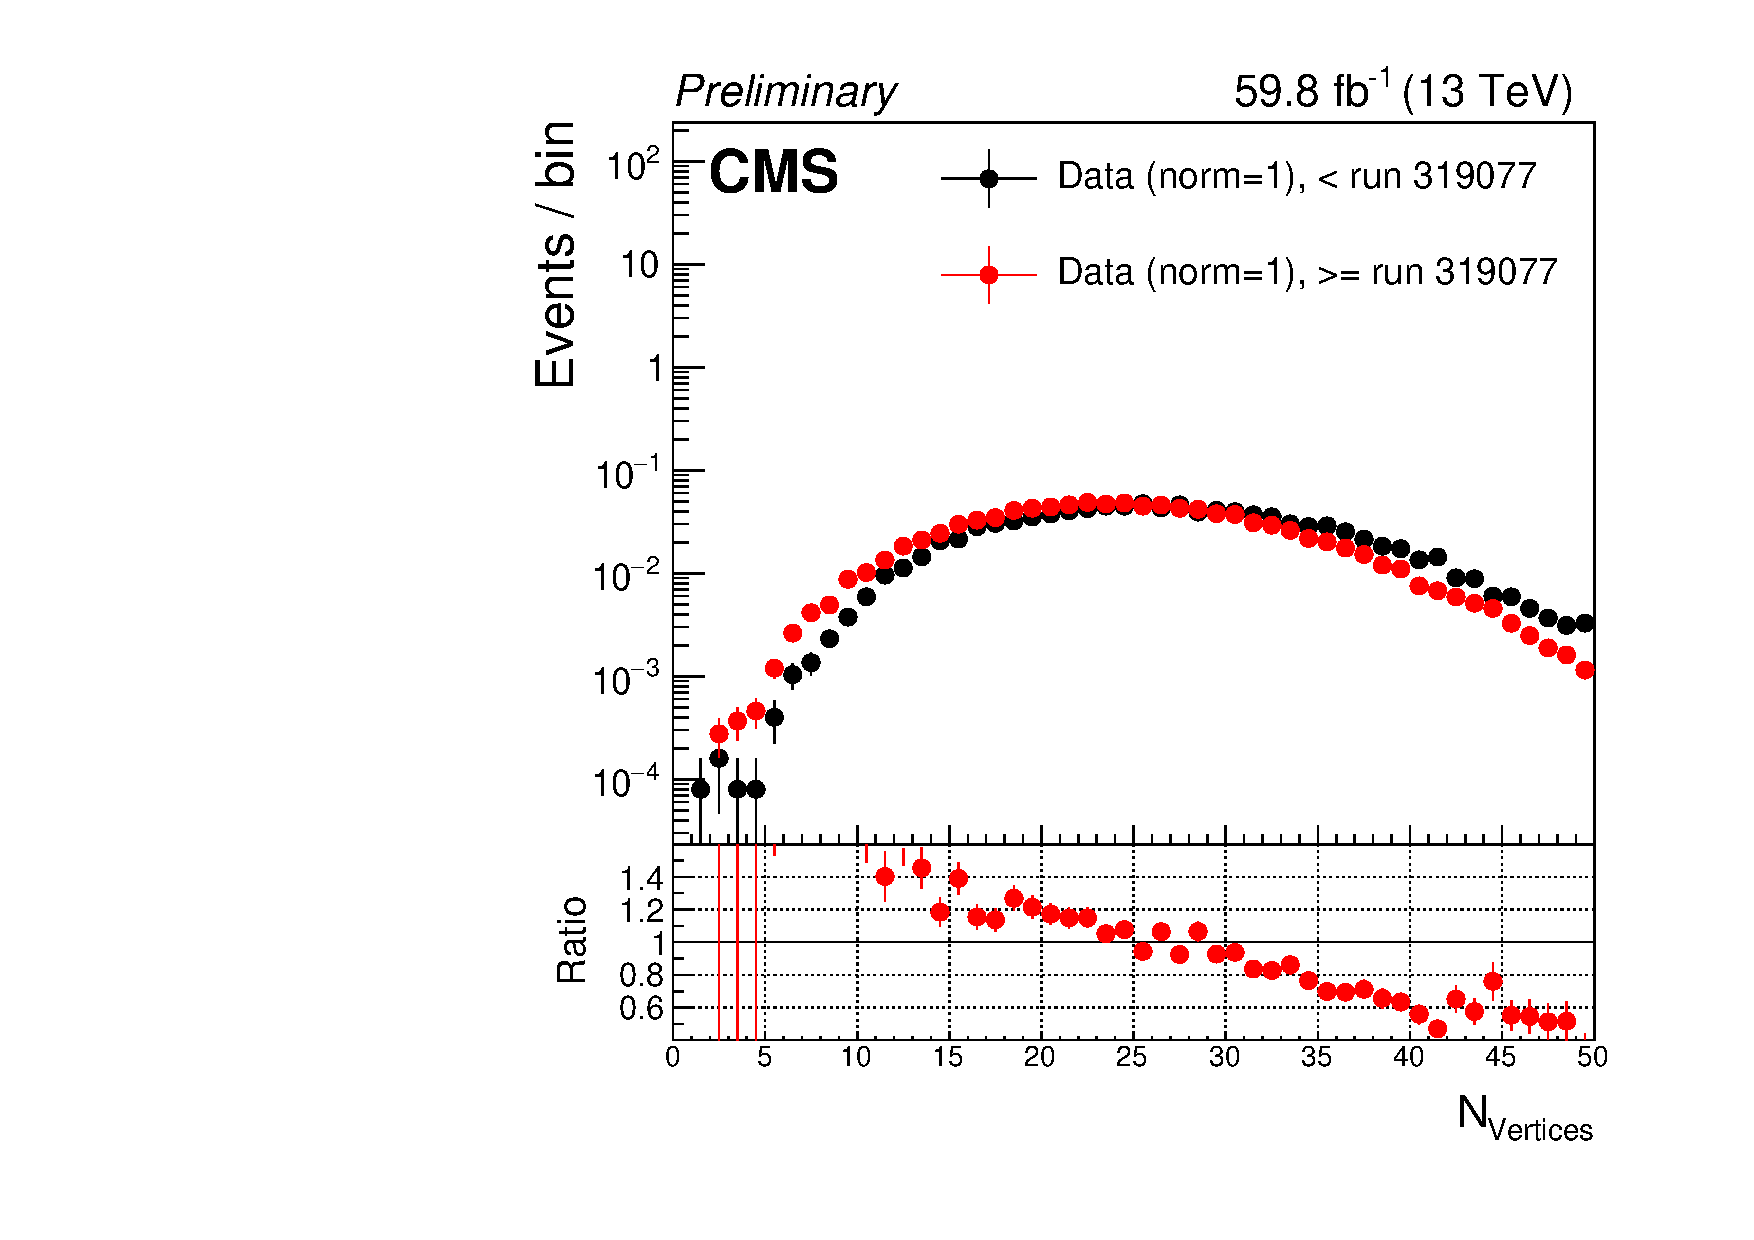
\includegraphics[width=.49\textwidth]{Images/Analysis/Results_HEMFailureStudyPlots_Data_BeforeAfterRun319077/BasicLQ_uujj_GoodVertexCount_linscale.pdf}}
    \caption{A shape comparison of 2018 data in periods A (black) and B (red). Data in each period have been normalized to unity and have preselection applied. The ratio \RatioDataAB is shown in the subplot. Vertical error bars represent the statistical uncertainty in each bin.}
    \label{figapp:hemvtx}
\end{figure}

\begin{figure}[H]
    \centering
    {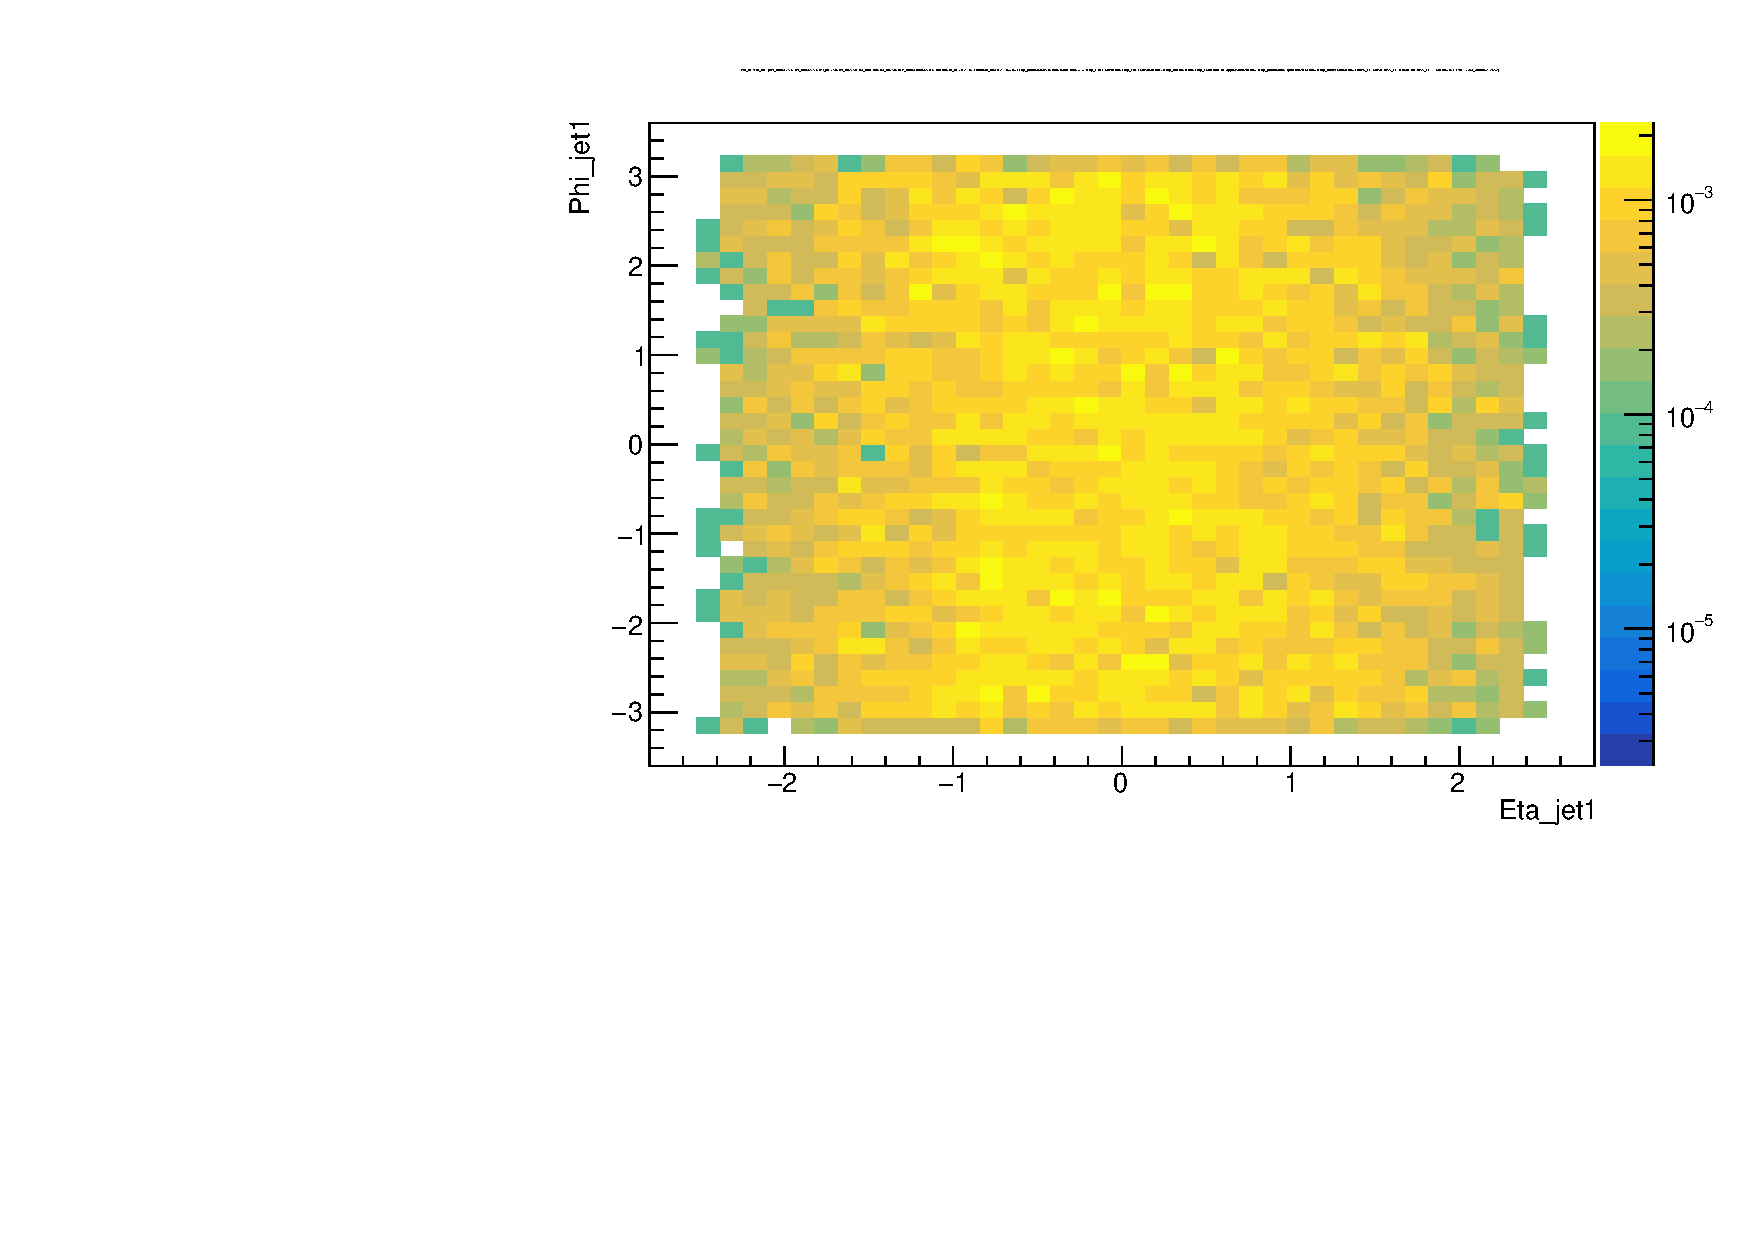
\includegraphics[width=.49\textwidth]{Images/Analysis/Results_HEMFailureStudyPlots_Data_BeforeAfterRun319077_JetOccupancy/Jet1_Phi_vs_Eta_BeforeRun319077.pdf}}
    {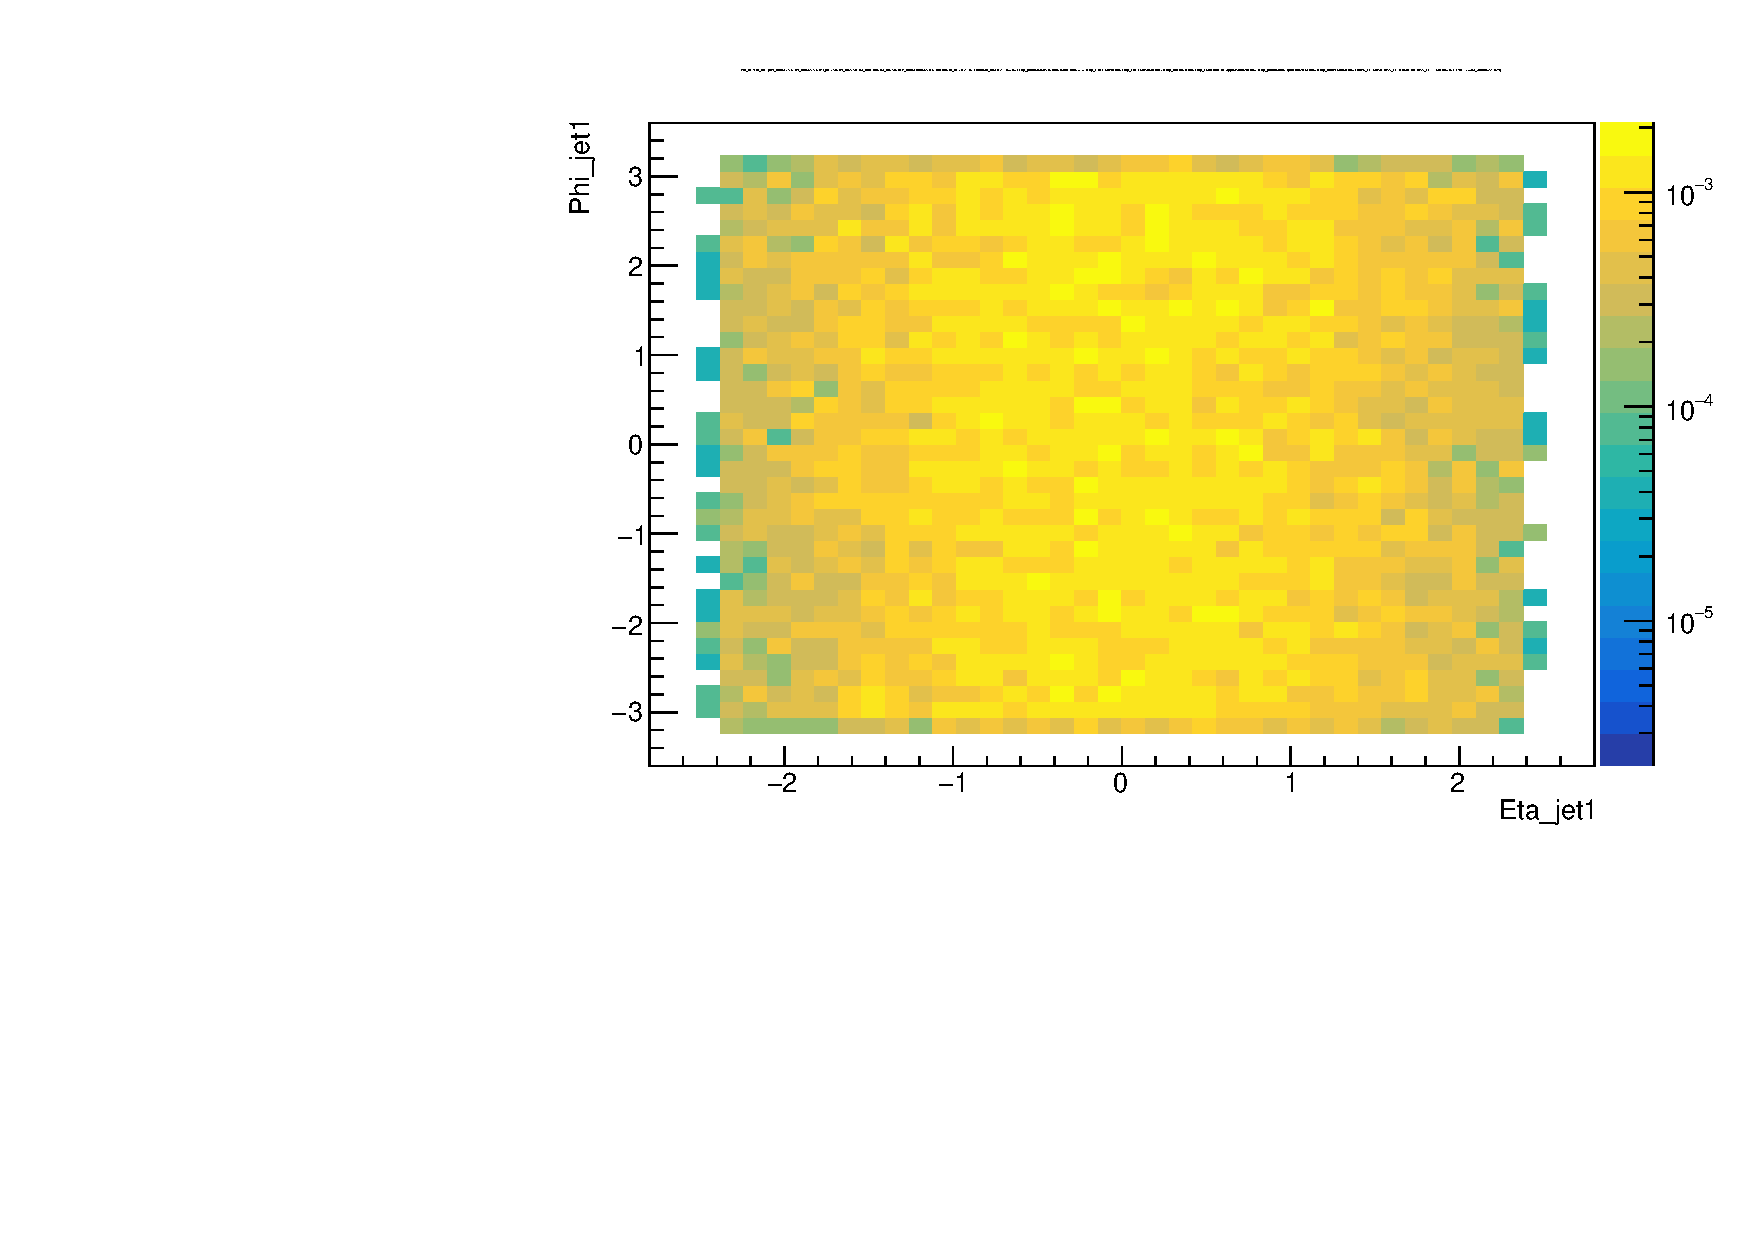
\includegraphics[width=.49\textwidth]{Images/Analysis/Results_HEMFailureStudyPlots_Data_BeforeAfterRun319077_JetOccupancy/Jet1_Phi_vs_Eta_AfterRun319077.pdf}}
    {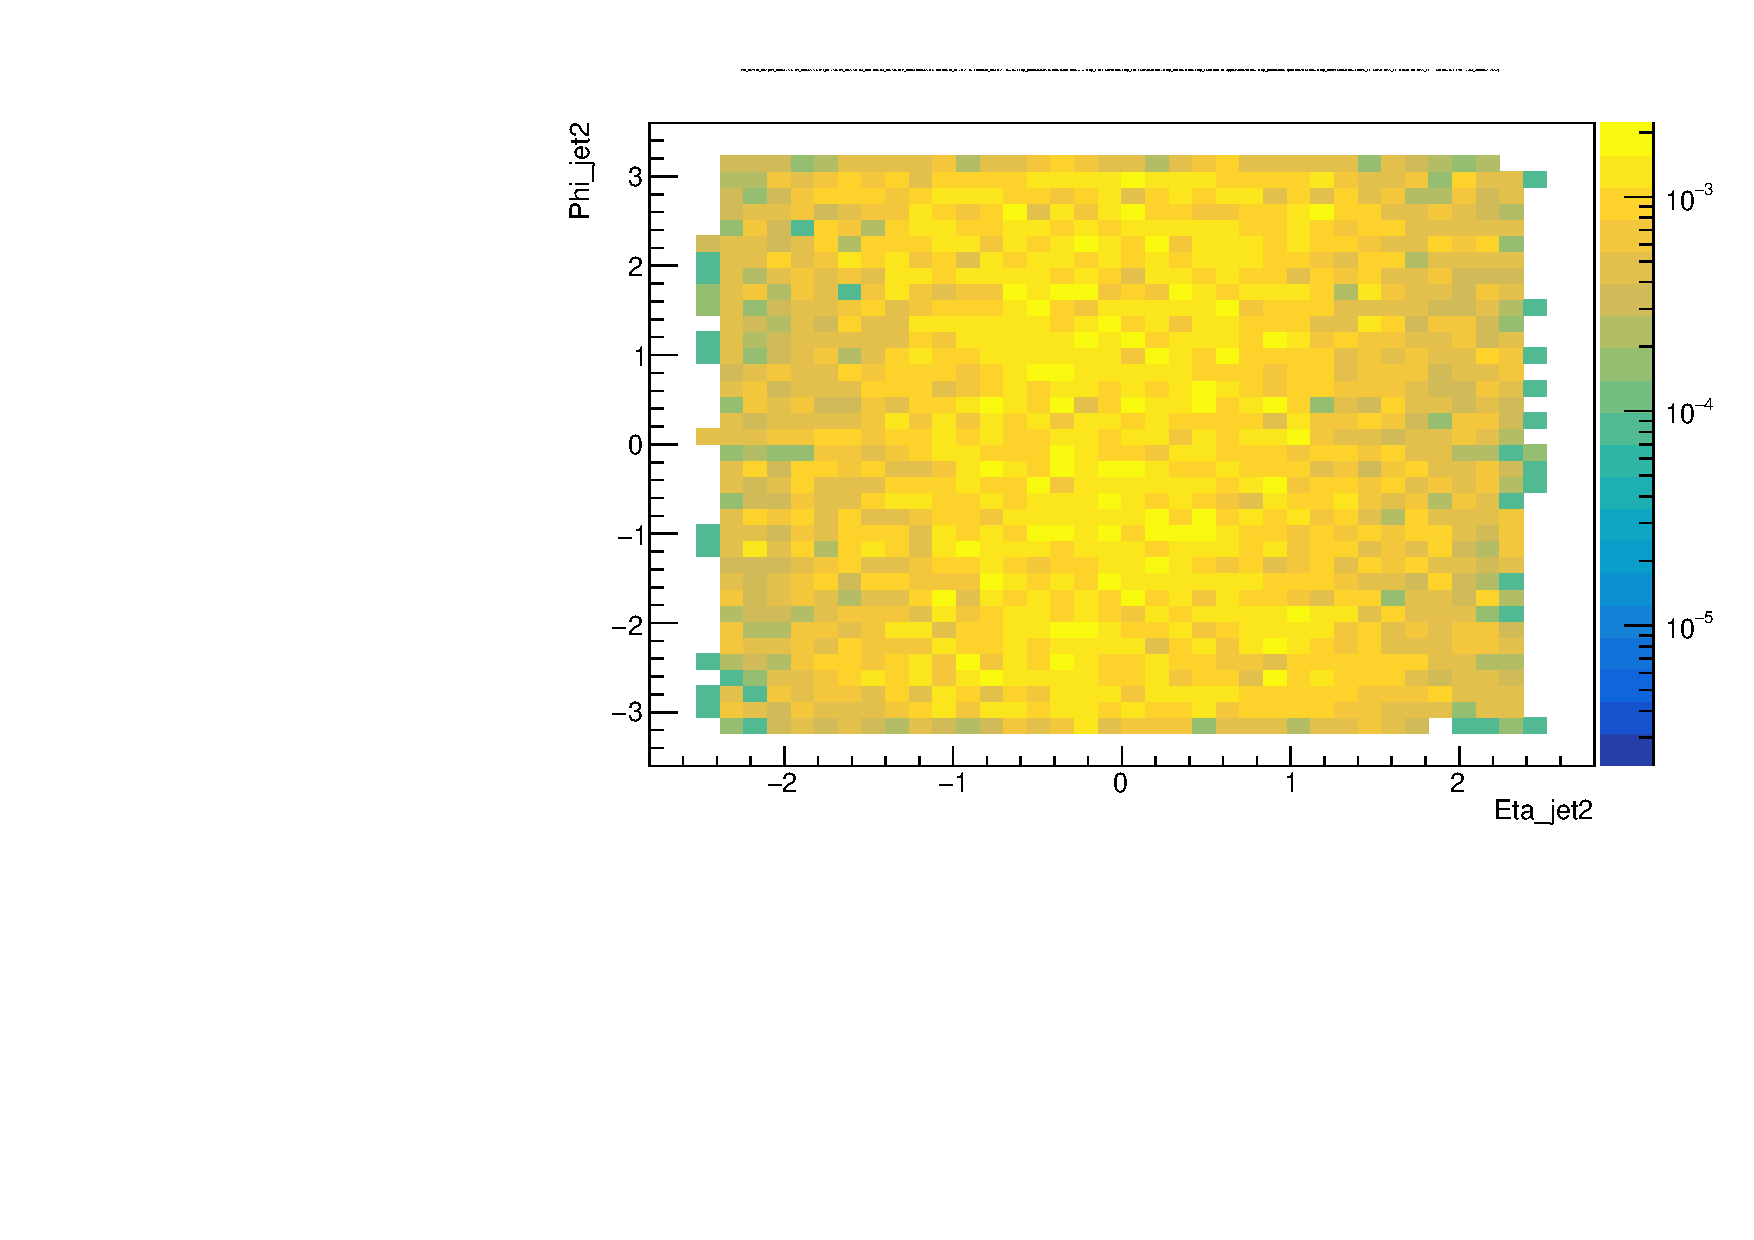
\includegraphics[width=.49\textwidth]{Images/Analysis/Results_HEMFailureStudyPlots_Data_BeforeAfterRun319077_JetOccupancy/Jet2_Phi_vs_Eta_BeforeRun319077.pdf}}
    {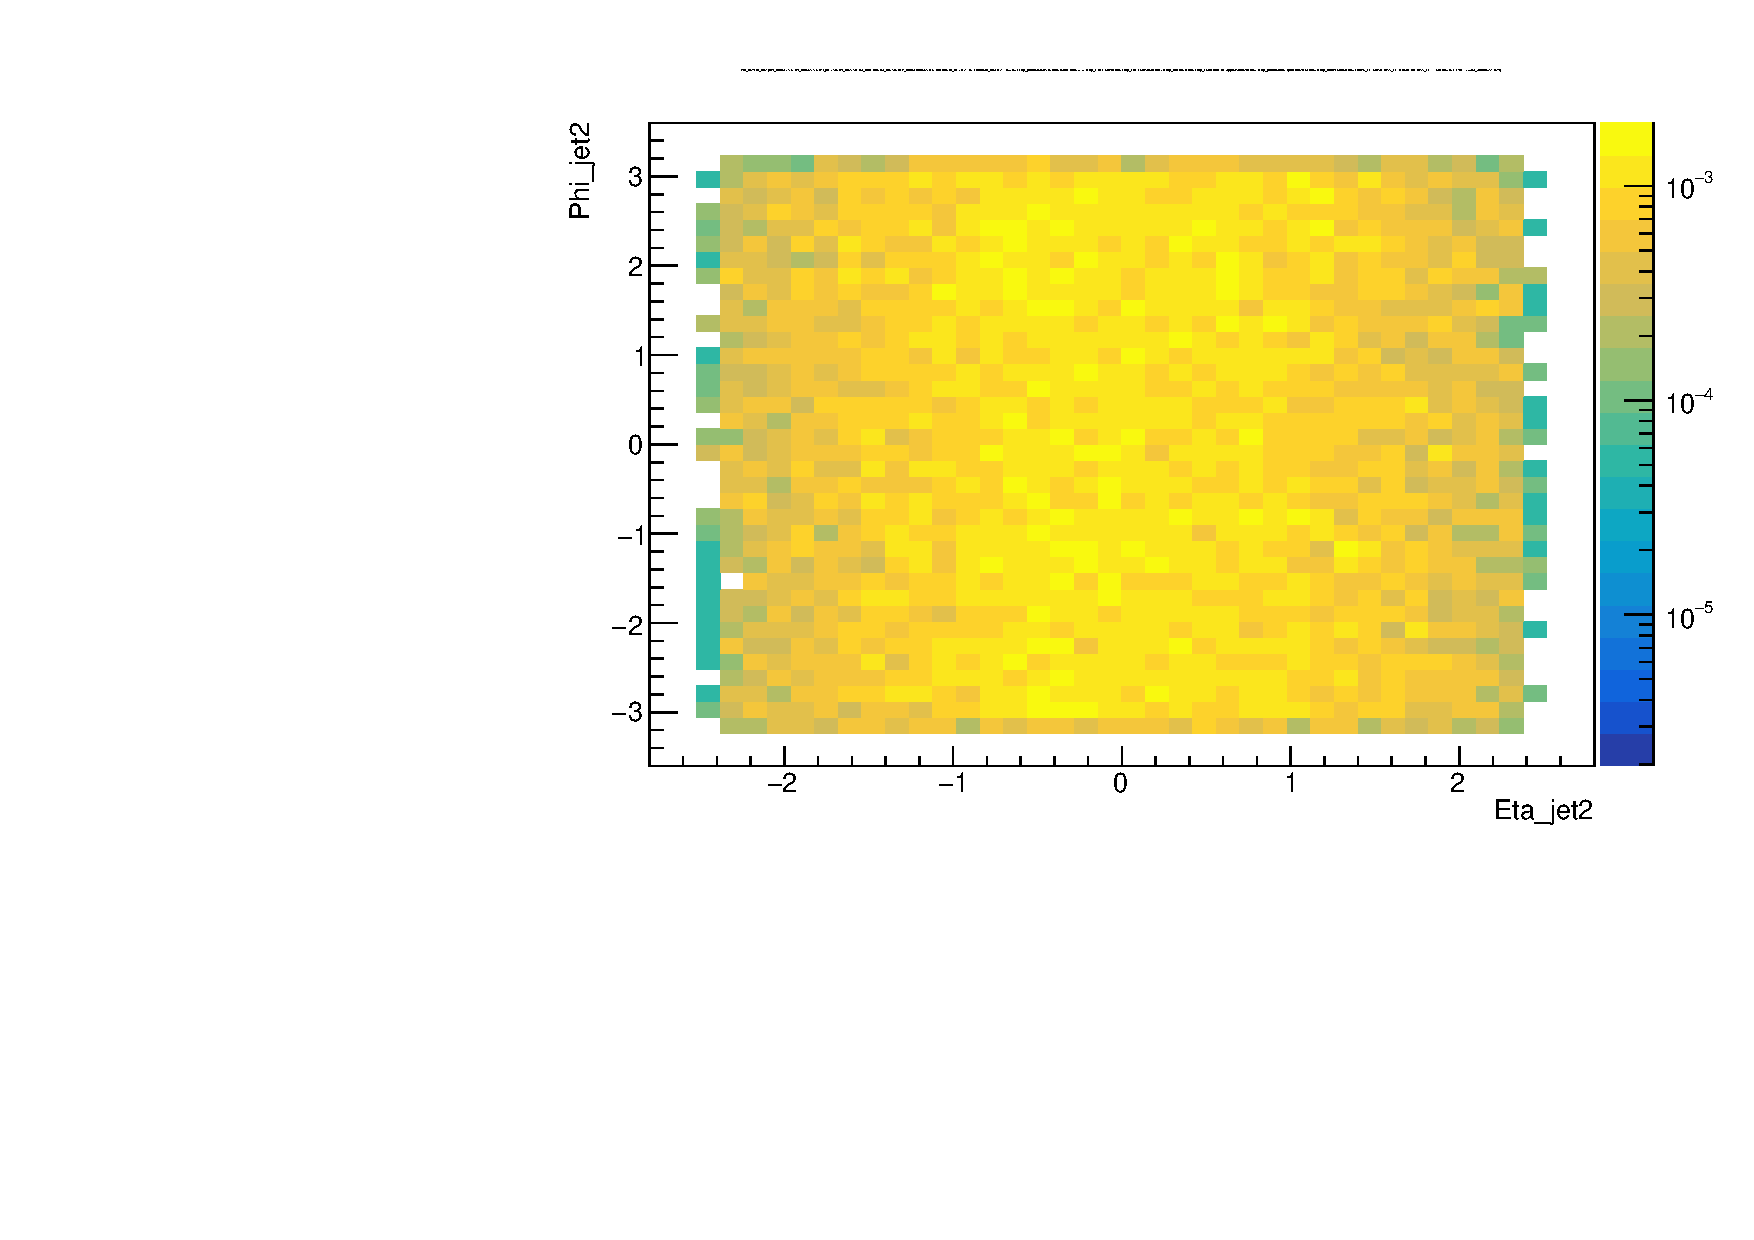
\includegraphics[width=.49\textwidth]{Images/Analysis/Results_HEMFailureStudyPlots_Data_BeforeAfterRun319077_JetOccupancy/Jet2_Phi_vs_Eta_AfterRun319077.pdf}}
    \caption{A comparison of 2018 data in periods A (left) and B (right) shown in jet occupancy. Data in each period have been normalized to unity and have preselection applied.}
    \label{figapp:hemjetoccupancy}
\end{figure}